%=================================================%
% Section:                        	              %
%    Results %
%=================================================%

\begin{center}
\section{Results}
\label{sec:Results}
\end{center}

%====================================================================%
% SubSection:                        	                             %
%    Results: Introduction %
%====================================================================%
\aboveSubSecSkip

\subsection{Introduction}
\label{sec:Results-Intro}

\noindent
	\indent This chapter contains the results obtained from the grey and frequency dependent calculations with and without the difference formulation. In the grey case, the numerical results are compared to the semianalytic Marshak wave benchmarks present by Su and Olson[Su 1996]. Frequency dependent calculations are compared to the non-grey semianalytic benchmarks also presented by Su and Olson[Su 1999]. Figures of merit are calculated for the different solution scenarios to evaluate the effectiveness of the variance reduction. The stability of the difference formulation for the diffusion equation is also explored in grey and frequency dependent systems. 
				
\belowSubSecSkip

%=====================================================================%
% SubSection:                        	                              %
%     Results:Grey Implicit Monte Carlo Diffusion %
%=====================================================================%
\subsection{Grey Implicit Monte Carlo Diffusion}
\label{sec:Grey}

\noindent
	\indent We first test the implementation of IMD on a one dimensional grey test problem[Gen 2001]. This problem consists of an initially cold semi-infinite body that has a flux incident on the left face. This problem has a normalized semi-analytic solution[Su 1996].  The Su and Olson results were translated into a normalized form to allow comparison with the IMD code results using the constants defined in Table \ref{table:constants}. The unit (Mm) denotes Mega meters (or 1e+6 meters).

\begin{table}[htbp]
	\begin{center}	
	\begin{tabular} {|c||c|c|c|c|} \hline
		\multicolumn{4}{|c|} {Constants} \\ [0.5ex]\hline
		Constant & Symbol & Value & Units \\ [0.5ex] \hline\hline
		\bf{\emph{Planck}} & $h$ & 6.626E-34 & joule*sec. \\ \hline
		\bf{\emph{Boltzmann}} & $k$ & 1.381E-23 & joule/Kelvin \\ \hline
		\bf{\emph{Speed of Light}} & $c$ & 299.8 & Mm/sec. \\ \hline
	\end{tabular}
	\caption{\label{table:constants} Constants used for all calculations}
	\end{center}
 \end{table}

	Two different approaches are used to solve the grey test problem: an optimized grey IMD code, and a multigroup IMD code that uses a constant frequency-independent opacity. The multigroup code with the difference formulation is significantly slower because of the necessity to integrate the frequency dependence of the differenced Plankian. It is also slower without the difference formulation because of sampling overhead.

%==================%
% SubSubSection:   %
%    Grey Without the Difference Formulation %
%==================%
\subsubsection{Grey without the Difference Formulation}
\label{sec:Grey_w/out_df}

	The first problem is the grey purely absorbing Su and Olson Marshak wave problem. This problem will be referred to as ``Problem 1.1''. The face source, which is constant over time and has a magnitude of 74.925 at x=0 and 0 every where else, is turned on at $\tau=0.0$ and left on for the duration of the problem, until $\tau=1.0$. The problem specification is included in Table \ref{table:Problem1.1}.

\begin{table}[htbp]
	\begin{center}	
	\begin{tabular} {|c||c|c|c|} \hline
		\multicolumn{3}{|c|} {Problem 1.1 Parameters} \\ [0.5ex]\hline
		Parameter & Value  & Units \\ [0.5ex] \hline\hline
		{{Number of Cells}} 	& 500 	& N/A \\ \hline
		{{Number of Particles}} & 4000 	& N/A \\ \hline
		{{Length}} 		& 50 	& Mm \\ \hline
		{{Left Albedo}} 	& 0 	& N/A \\ \hline
		{{Right Albedo}} 	& 1 	& N/A \\ \hline
		{{Initial Material Temp.}} & 0.01 & K \\ \hline
		{{Material Density}} 	& 1.0 	& Kg/Mm \\ \hline
		{{Number Of Time Steps}}& 20 	& N/A \\ \hline
		{{Final Time [$\tau$]}} & 1.0 	& N/A \\ \hline
		{{Material Opacity}} 	& 1.0 	& 1/Mm \\ \hline
	\end{tabular}
	\caption{\label{table:Problem1.1} Problem specifications used for the Su and Olson purely absorbing grey Marshak wave problem (Problem 1.1)}
	\end{center}
 \end{table}

\noindent \begin{figure}[htbp]
	\unitlength1in
	\begin{center}
		\begin{minipage}[t]{6in}
		\centering
		\begin{picture}(\width,\height)
	                {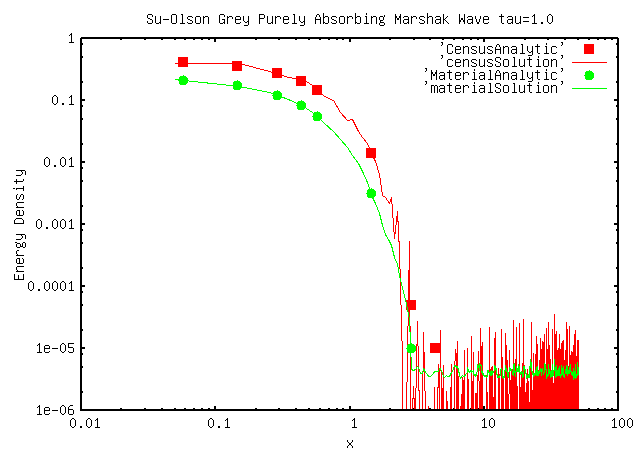
\includegraphics[width=\imgwidth,height=\imgheight]{Grey_MW_No_DF_L=50}}
		\end{picture}
		\caption{\label{fig:Grey_MW_No_DF_L=50} Normalized one dimensional grey solution compared to Su and Olson result[Su 1996] at $\tau=1.0$ with no scattering and no difference formulation. (Problem 1.1)}
		\end{minipage} \hfill
	\end{center}
\end{figure}

 	Figure \ref{fig:Grey_MW_No_DF_L=50} demonstrates the results obtained from the optimized grey IMD code. In this figure ``censusSolution'' denotes the photon energy density as determined by the IMD method, ``CensusAnalytic'' represents the semi-analytic benchmark results from Su and Olson, ``materialSolution'' denotes the material energy density calculated via the IMD method and finally ``MaterialAnalytic'' is the semi-analytic material energy density benchmark results from Su and Olson.

	The results from the multigroup calculation of this test problem are shown in Figure \ref{fig:Grey_MG_MW_No_DF_L=50}.

\begin{figure}[htbp]
	\unitlength1in
	\begin{center}
		\begin{minipage}[t]{6in}
		\centering
		\begin{picture}(\width,\height)
	                {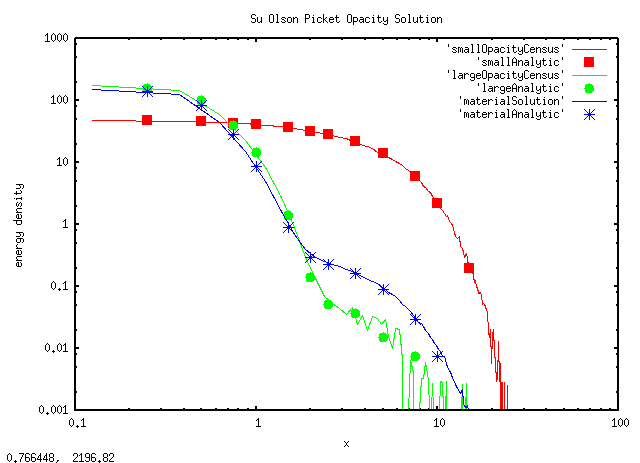
\includegraphics[width=\imgwidth,height=\imgheight]{Grey_MG_MW_No_DF_L=50}}
		\end{picture}
		\caption{\label{fig:Grey_MG_MW_No_DF_L=50} Grey IMD solution run with the multigroup IMD code compared to Su and Olson result[Su 1996]. (Problem 1.1)}
		\end{minipage} %\hfill
	\end{center}
\end{figure}

	Next, the effect of spatial (Problem 1.2a) and temporal (Problem 1.2b) refinement was investigated with the grey IMD code. This problem will be referred to as ``Problem 1.2''. Five versions of this test problem were run for each type of refinement. The spatial refinement was tested using the basic run settings defined in Table \ref{table:Problem1.2a}.  The different spatial refinements are listed in Table \ref{table:Problem1.2Spaital}.

\begin{table}[htbp]
	\begin{center}	
	\begin{tabular} {|c||c|c|c|} \hline
		\multicolumn{3}{|c|} {Problem 1.2 Parameters} \\ [0.5ex]\hline
		Parameter & Value  & Units \\ [0.5ex] \hline\hline
		{{Number of Cells}} 	& 120 	& N/A \\ \hline
		{{Number of Particles}} & 10000 	& N/A \\ \hline
		{{Length}} 		& 15 	& Mm \\ \hline
		{{Left Albedo}} 	& 0 	& N/A \\ \hline
		{{Right Albedo}} 	& 1 	& N/A \\ \hline
		{{Initial Material Temp.}} & 0.01 & K \\ \hline
		{{Material Density}} 	& 1.0 	& Kg/Mm \\ \hline
		{{Number Of Time Steps}}& 20 	& N/A \\ \hline
		{{Final Time [$\tau$]}} & 1.0 	& N/A \\ \hline
		{{Material Opacity}} 	& 1.0 	& 1/Mm \\ \hline
	\end{tabular}
	\caption{\label{table:Problem1.2a} Problem specifications used for Problem 1.2.}
	\end{center}
 \end{table}

\begin{table}[htbp]
	\begin{center}	
	\begin{tabular} {|c|c|} \hline
		\multicolumn{2}{|c|} {Problem 1.2a Spatial Refinements} \\ [0.5ex]\hline
		Number of Cells & Cell Size \\ [0.5ex] \hline\hline
		60  & 0.25  \\ \hline
		120 & 0.125	 \\ \hline
		240 & 0.0625	 \\ \hline
		480 & 0.03125	 \\ \hline
		960 & 0.015625  \\ \hline
	\end{tabular}
	\caption{\label{table:Problem1.2Spaital} Spatial refinements for Problem 1.2a}
	\end{center}
 \end{table}

\begin{figure}[htbp]
	\unitlength1in
	\begin{center}
		\begin{minipage}[t]{6in}
		\centering
		\begin{picture}(\width,\height)
	                {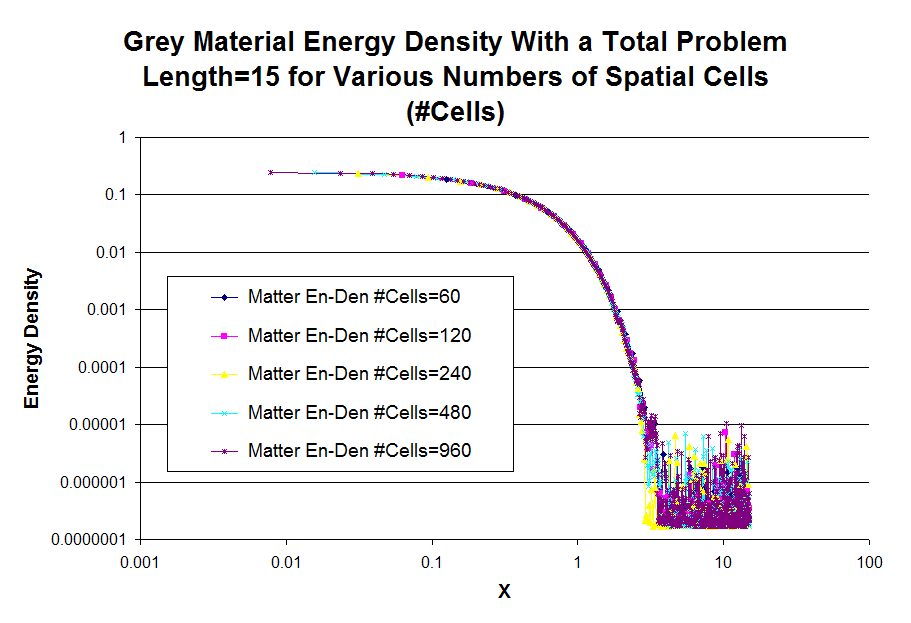
\includegraphics[width=\imgwidth,height=\imgheight]{G-Refine-Space}}
		\end{picture}
		\caption{\label{fig:Grey-Spatial-Refinment} Material energy densities from the grey IMD code with various cell sizes. (Problem 1.2a)}
		\end{minipage} %\hfill
	\end{center}
\end{figure}

	
	Figure \ref{fig:Grey-Spatial-Refinment} demonstrates the material energy density determined by the grey IMD code for various cell sizes. This shows that spatial refinement has very little relative effect on the shape of the material energy density.

	The temporal refinement for Problem 1.2 was performed using settings identical to those described in Table \ref{table:Problem1.2a}. Table \ref{table:Problem1.2Tempral} lists the five temporal refinements that were considered.

\begin{table}[htbp]
	\begin{center}	
	\begin{tabular} {|c|c|} \hline
		\multicolumn{2}{|c|} {Problem 1.2b Temporal Refinements} \\ [0.5ex]\hline
		Number of Time Steps & Time Step Size $\Delta{\tau}$ \\ [0.5ex] \hline\hline
		 10  & 0.1      \\ \hline
		 120 & 0.05     \\ \hline
		 240 & 0.025    \\ \hline
		 480 & 0.0125   \\ \hline
		 960 & 0.00625  \\ \hline
	\end{tabular}
	\caption{\label{table:Problem1.2Tempral} Temporal refinements for Problem 1.2b}
	\end{center}
 \end{table}

\begin{figure}[htbp]
	\unitlength1in
	\begin{center}
		\begin{minipage}[t]{6in}
		\centering
		\begin{picture}(\width,\height)
	                {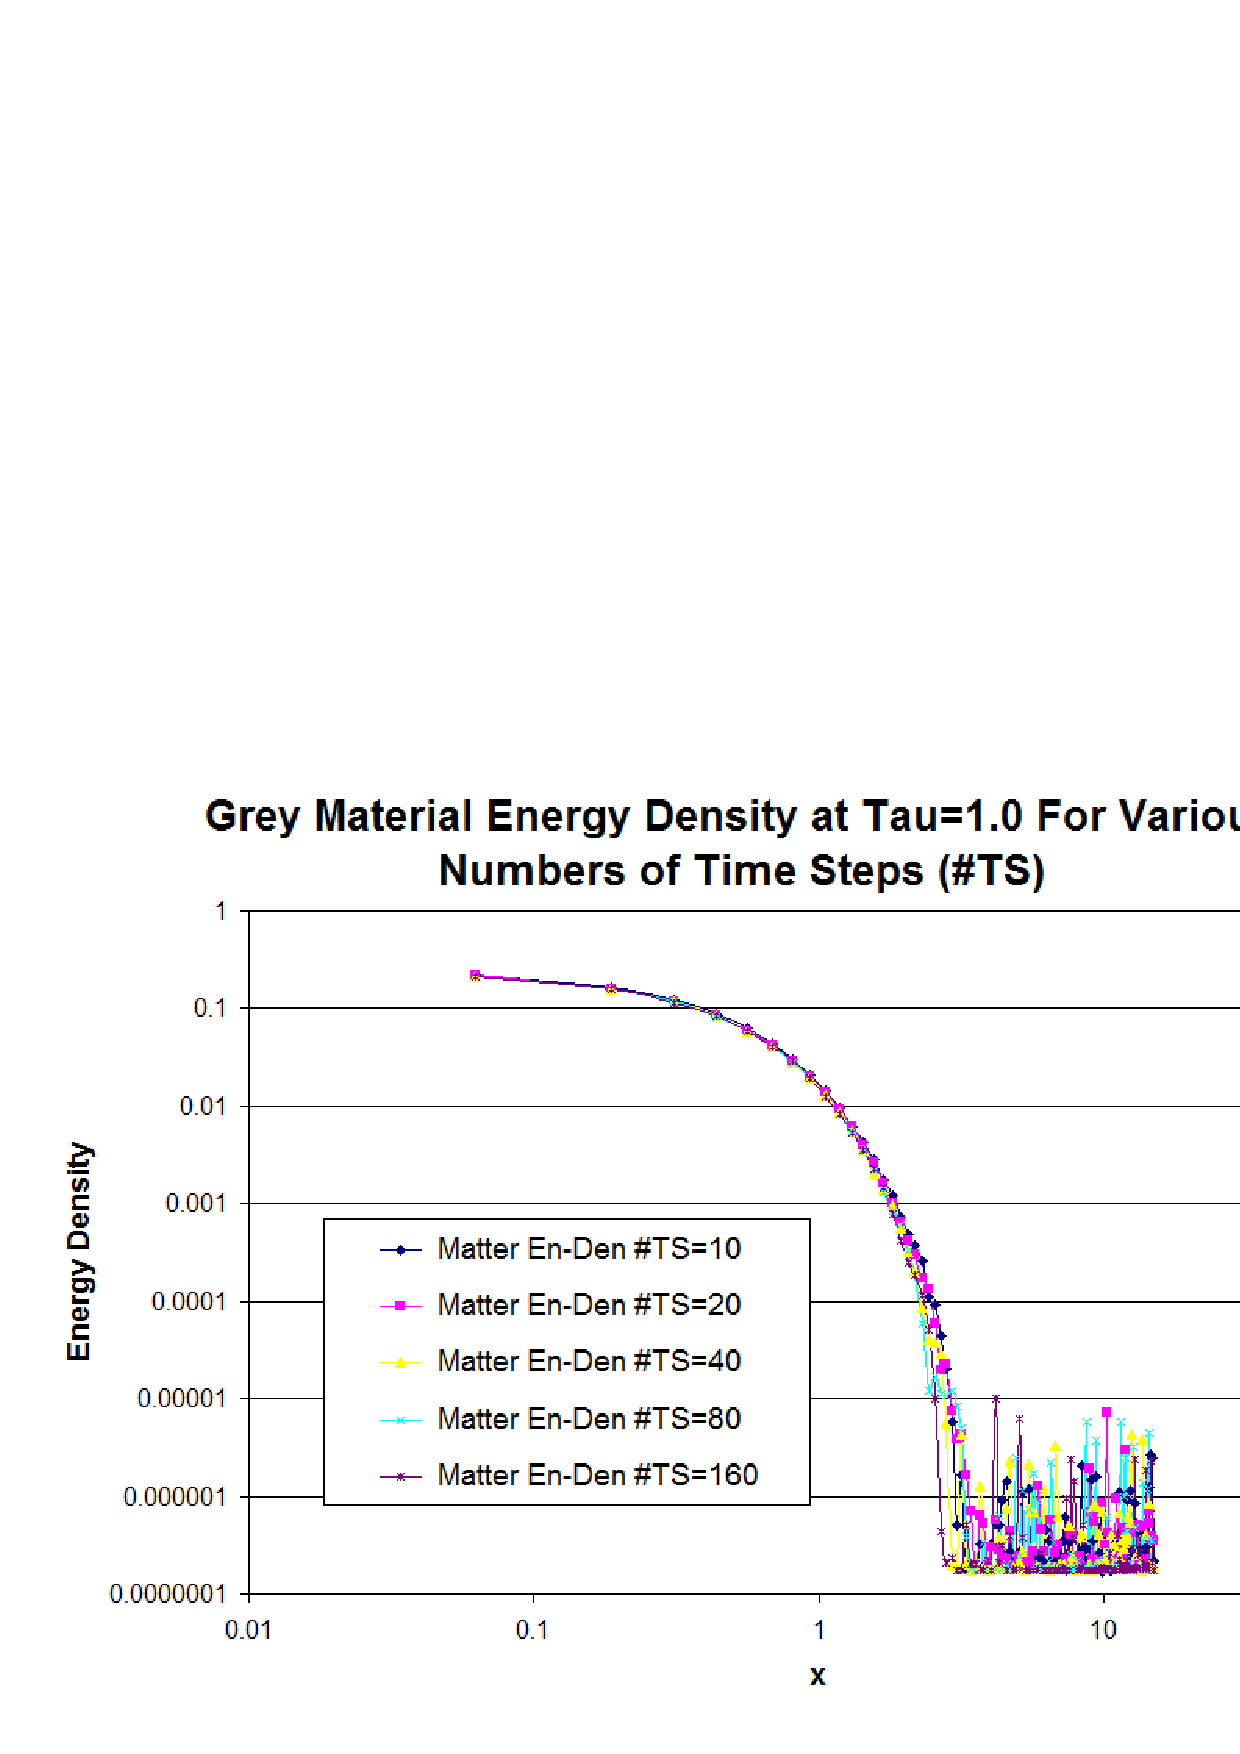
\includegraphics[width=\imgwidth,height=\imgheight]{G-Refine-time}}
		\end{picture}
		\caption{\label{fig:Grey-Tempral-Refinment1} Material energy densities from the grey IMD code with various time step sizes. (Problem 1.2b)}
		\end{minipage} %\hfill
	\end{center}
\end{figure}

\begin{figure}[htbp]
	\unitlength1in
	\begin{center}
		\begin{minipage}[t]{6in}
		\centering
		\begin{picture}(\width,\height)
	                {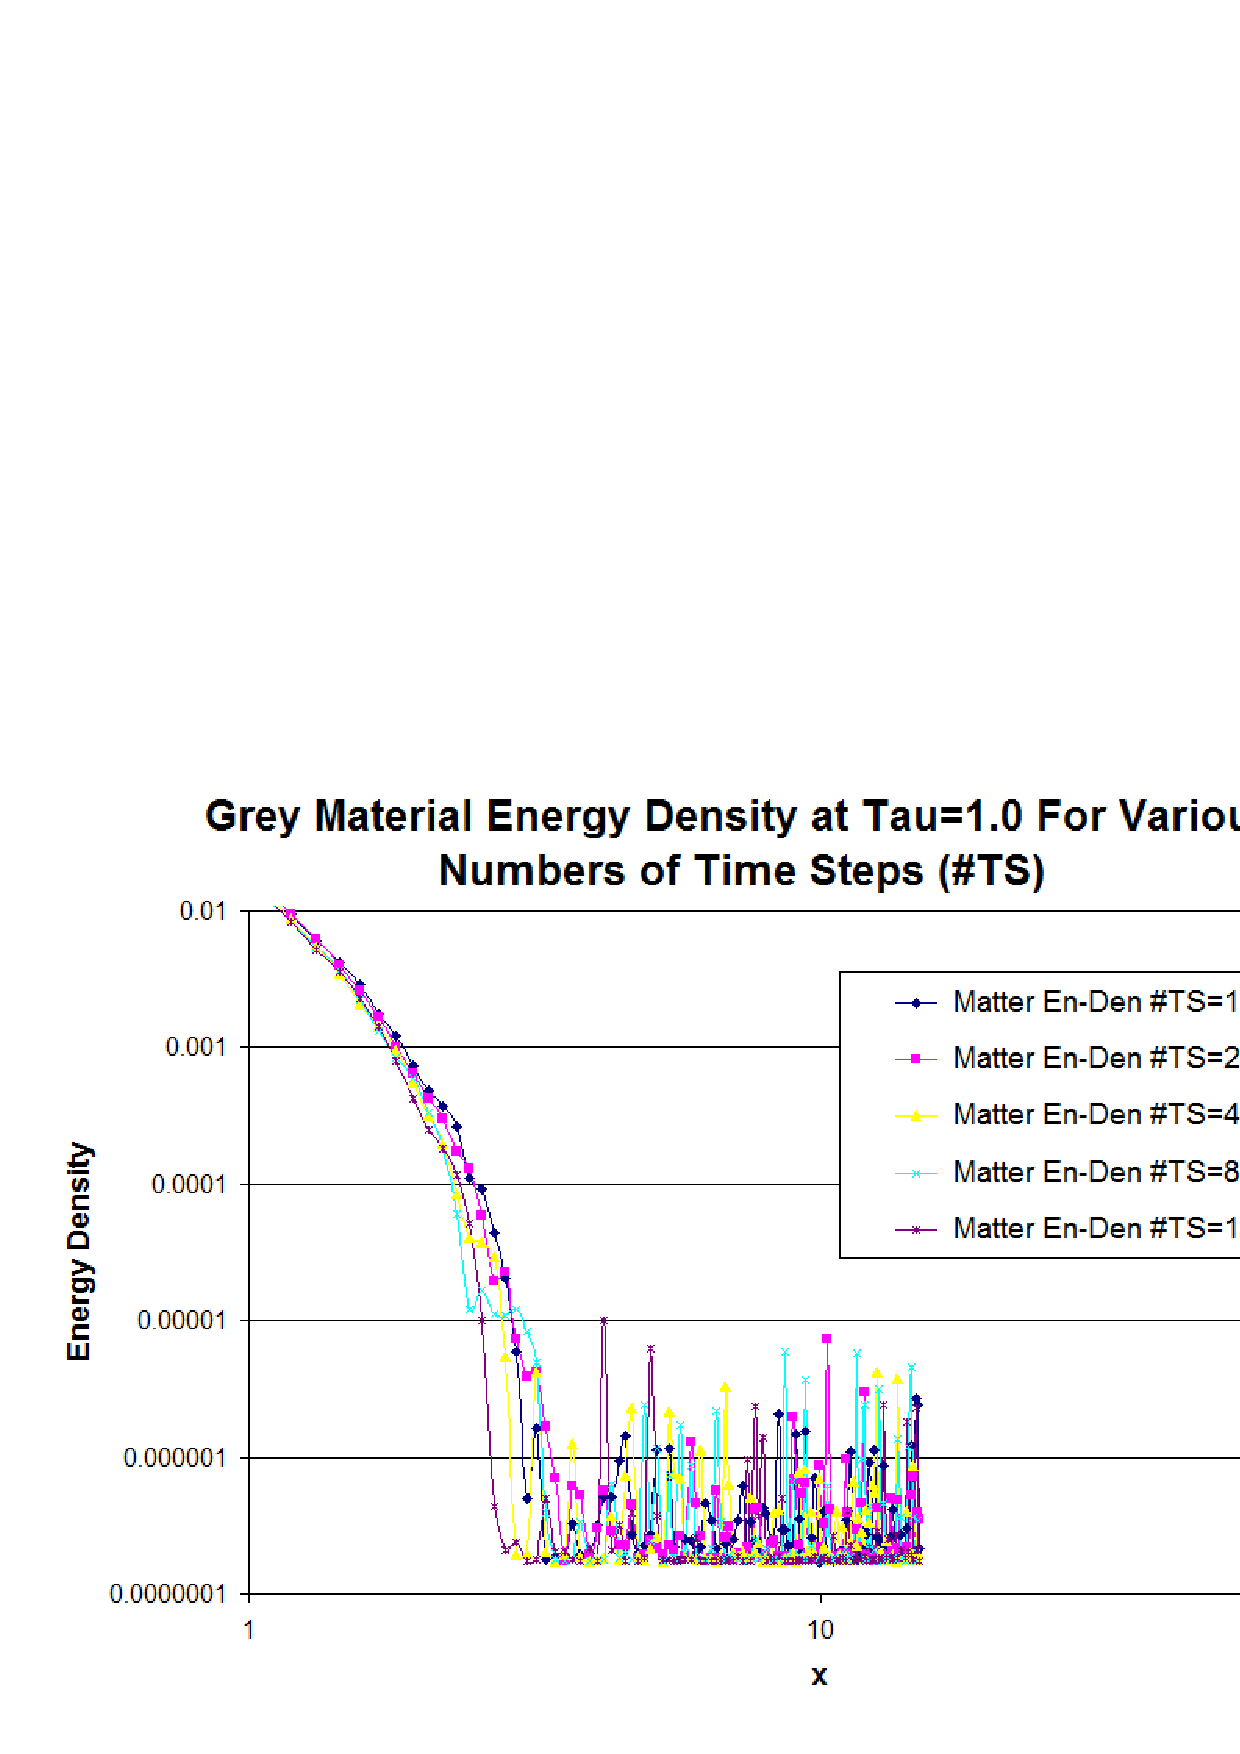
\includegraphics[width=\imgwidth,height=\imgheight]{G-Refine-time2}}
		\end{picture}
		\caption{\label{fig:Grey-Tempral-Refinment2} A closer look at the leading edge of the Marshak wave material energy densities from the grey IMD code with various time step sizes. (Problem 1.2b)}
		\end{minipage} %\hfill
	\end{center}
\end{figure}

	Figures \ref{fig:Grey-Tempral-Refinment1} and \ref{fig:Grey-Tempral-Refinment2} show that the degree of temporal refinement has a greater effect on the numerical solution than the degree of the spatial refinement. This is paticularly true at the leading edge of the Marshak wave.
%==================%
% SubSubSection:   %
%    Grey Without the Difference Formulation %
%==================%
\subsubsection{Grey with the Difference Formulation}
\label{sec:Grey_w/df}

	In Problem 1.2, the Su and Olson grey benchmark result is simulated using the optimized grey IMD code and the difference formulation. In this case, the difference formulation temperature was chosen to be the material temperature in the associated cell. This problem has parameters identical to those of Problem 1.1 (see Table \ref{table:Problem1.1}).

\begin{figure}[htbp]
	\unitlength1in
	\begin{center}
		\begin{minipage}[t]{6in}
		\centering
		\begin{picture}(\width,\height)
	                {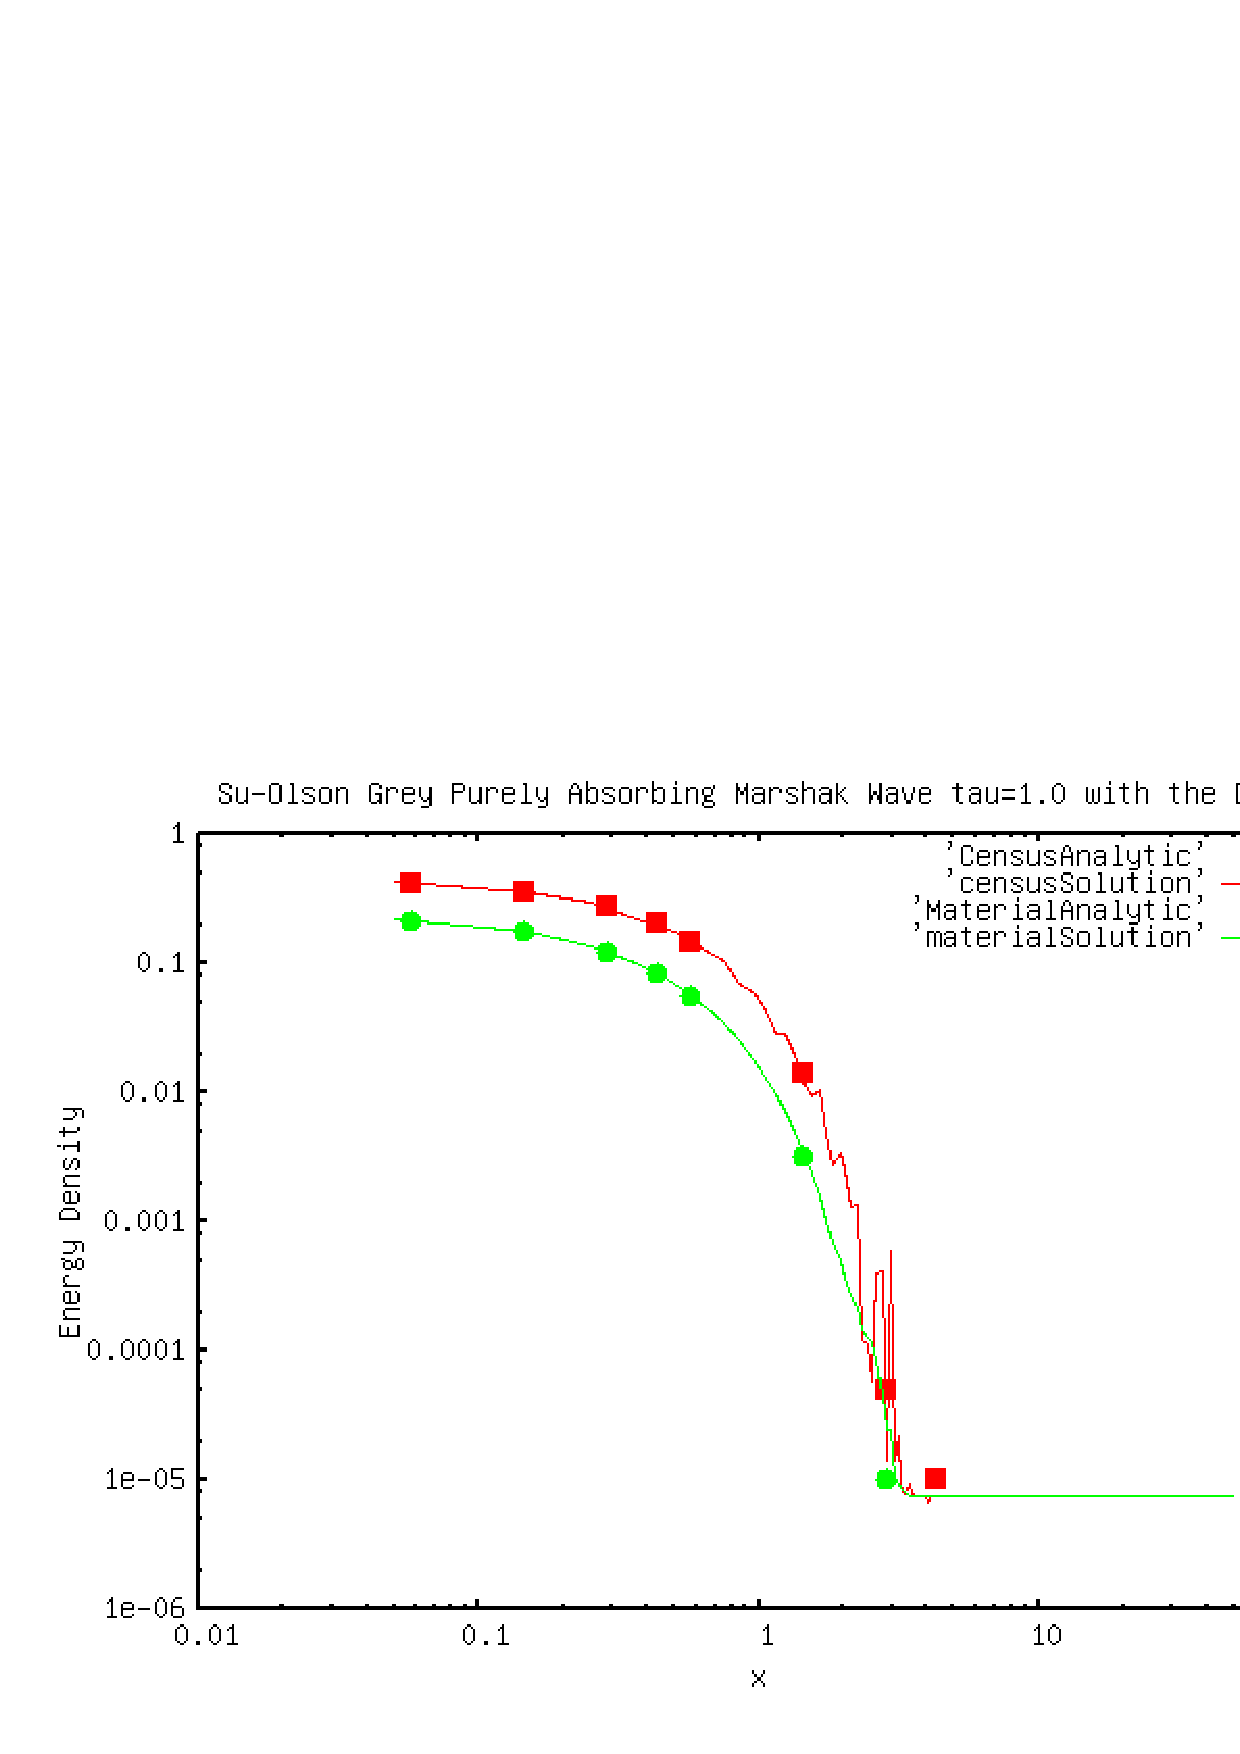
\includegraphics[width=\imgwidth,height=\imgheight]{Grey_MW_DF_L=50}}
		\end{picture}
		\caption{\label{fig:Grey_MW_DF_L=50} Normalized one dimensional grey solution  with the difference formulation compared to Su and Olson result[Su 1996] at $\tau=1.0$ with no scattering. (Problem 1.1)}
		\end{minipage} %\hfill
	\end{center}
\end{figure}

	The difference between figures \ref{fig:Grey_MW_DF_L=50} and \ref{fig:Grey_MW_No_DF_L=50} show that the difference formulation yields a significant reduction in the variance.

\belowSubSecSkip

%=====================================================================%
% SubSection:                        	                              %
%     Results: Markov-Markov Mixing Statistics - Vacuum Boundaries %
%=====================================================================%
\subsection{Frequency Dependent Implicit Monte Carlo Diffusion}
\label{sec:Results-MM-V}

\noindent
	\indent This section contains the results of test problems solved using the frequency dependent IMD method. This includes an exploration of frequency dependent systems with and without the difference formulation. The majority of the simulated results are compared against the Su and Olson non-grey Marshak wave semi-analytic benchmark with a picket fence opacity. The stability and accuracy of the method are investigated as both the number of time steps and the number of cells is varied. 

%==================%
% SubSubSection:   %
%    Grey Without the Difference Formulation %
%==================%
\subsubsection{Frequency Dependent IMD without the Difference Formulation}
\label{sec:Grey_w/out_df}

	The next problem is the Su and Olson non-grey benchmark result with a picket fence opacity defined such that: the bins are logarithmically spaced in frequency, even frequency bins have a large opacity, and odd frequency bins have a small opacity. The opacities are chosen such that the Planck opacity, defined by equation \ref{PlanckOpacity2}, is equal to one[Su 1999]. The opacities chosen for this work are shown in Table \ref{table:opacities}

\begin{table}[htbp]
	\begin{center}	
	\begin{tabular} {|c||c|} \hline
		\multicolumn{2}{|c|} {Picket Fence Opacities} \\ [0.5ex]\hline
		Number of Time Steps & Time Step Size $\Delta{\tau}$ \\ [0.5ex] \hline\hline
		 Small Opacity  & ${2\over{101}}$      \\ \hline
		 Large Opacity  & ${200\over{101}}$      \\ \hline
	\end{tabular}
	\caption{\label{table:opacities} Opacities used to construct the opacity distribution for the frequency dependent IMD results.}
	\end{center}
 \end{table}

	The remainder of the specifications for this problem (Problem 3.1) are listed in Table \ref{table:Problem2.1}.

\begin{table}[htbp]
	\begin{center}	
	\begin{tabular} {|c||c|c|c|} \hline
		\multicolumn{3}{|c|} {Problem 3.1 Parameters} \\ [0.5ex]\hline
		Parameter & Value  & Units \\ [0.5ex] \hline\hline
		{{Number of Cells}} 	& 120 	& N/A \\ \hline
		{{Number of Particles}} & 400000 & N/A \\ \hline
		{{Length}} 		& 15 	& Mm \\ \hline
		{{Left Albedo}} 	& 1 	& N/A \\ \hline
		{{Right Albedo}} 	& 1 	& N/A \\ \hline
		{{Initial Material Temp.}} & 0.01 & K \\ \hline
		{{Material Density}} 	& 1.0 	& Kg/Mm \\ \hline
		{{Number Of Time Steps}}& 40 	& N/A \\ \hline
		{{Final Time [$\tau$]}} 	& 1.0 	& N/A \\ \hline
		{{Small Opacity}} 	& ${2\over{101}}$  & 1/Mm \\ \hline
		{{Large Opacity}} 	& ${200\over{101}}$  & 1/Mm \\ \hline
	\end{tabular}
	\caption{\label{table:Problem2.1} Problem specifications used for the Su and Olson purely absorbing grey Marshak wave problem at $\tau=1.0$ (Problem 3.1).}
	\end{center}
 \end{table}

\begin{figure}[htbp]
	\unitlength1in
	\begin{center}
		\begin{minipage}[t]{6in}
		\centering
		\begin{picture}(\width,\height)
	                {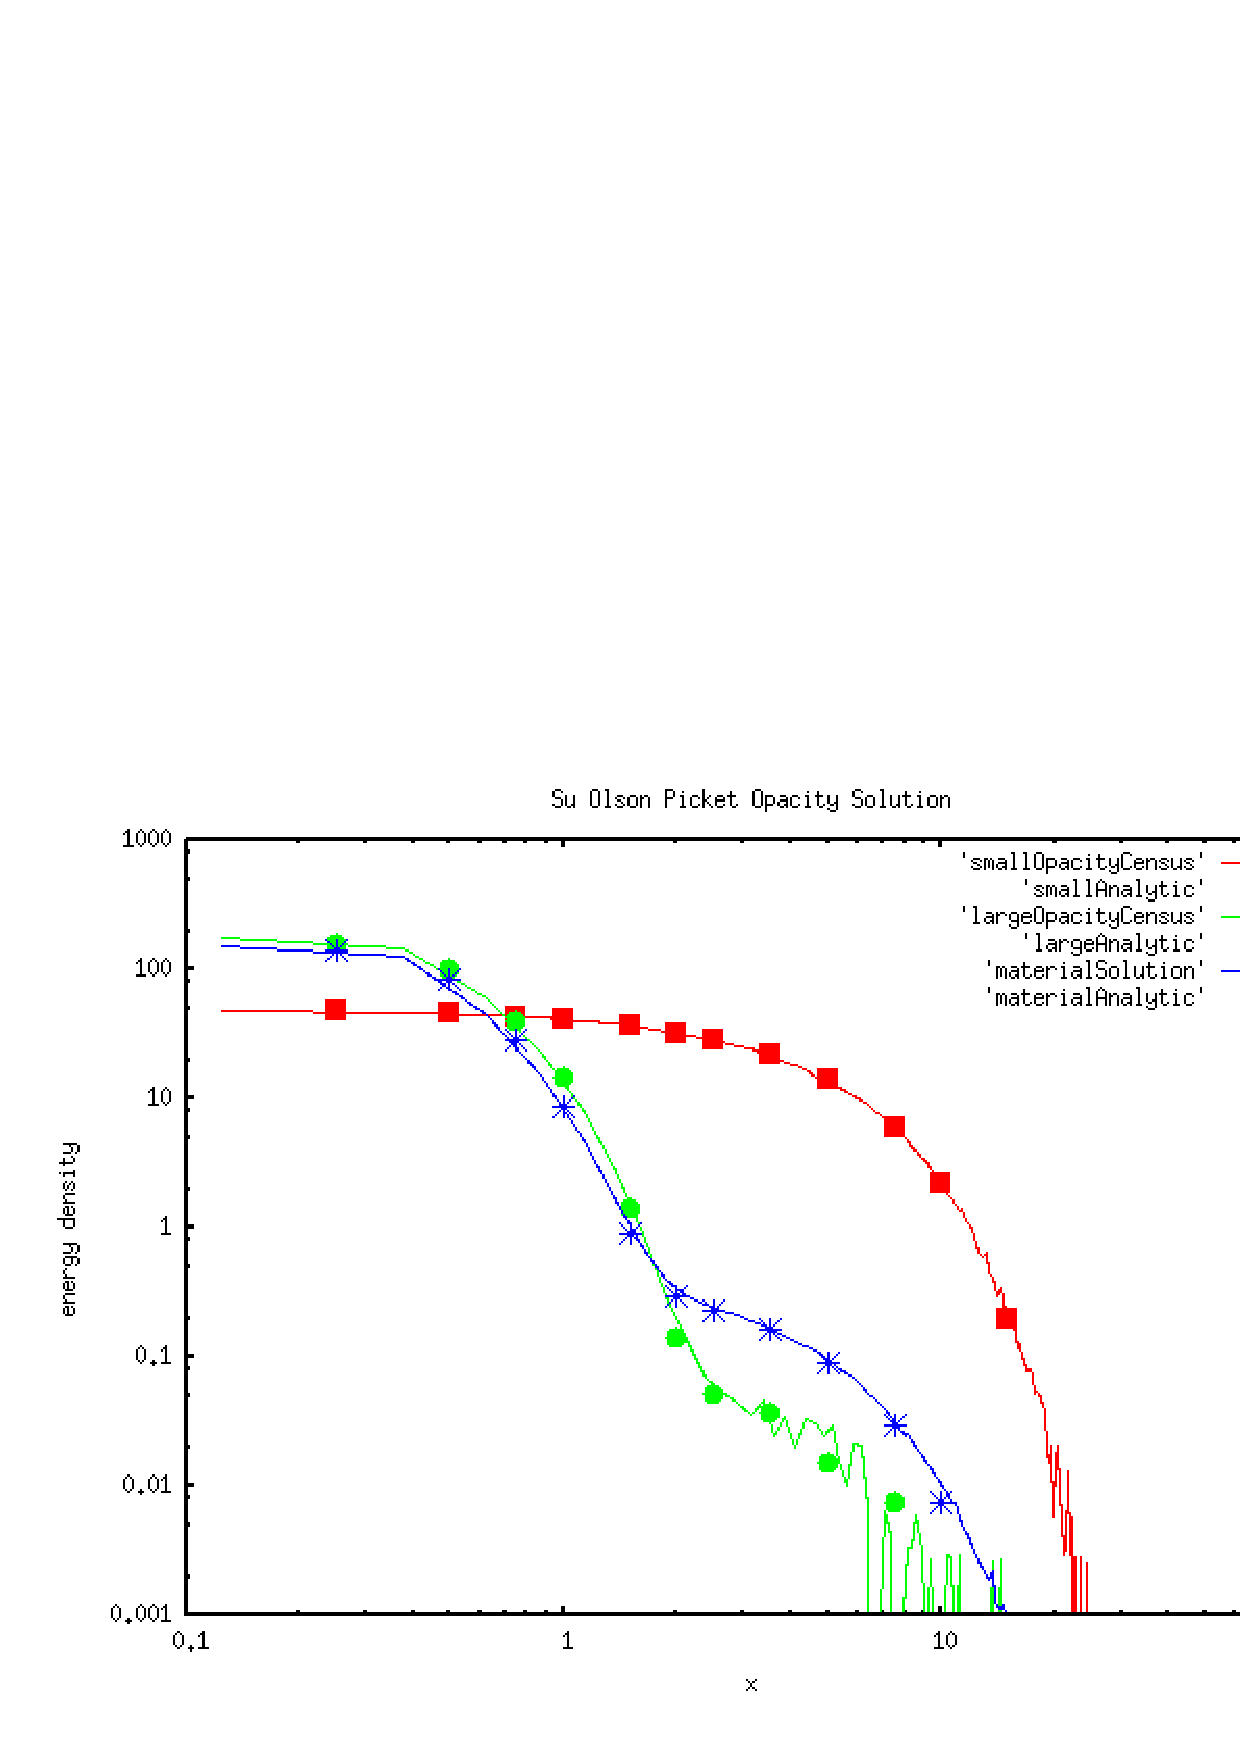
\includegraphics[width=\imgwidth,height=\imgheight]{NG-SO}}
		\end{picture}
		\caption{\label{fig:NG-SO} Normalized one dimensional frequency dependent solution compared to Su and Olson result[Su 1999] at $\tau=1.0$ with no difference formulation. (Problem 3.1)}
		\end{minipage} %\hfill
	\end{center}
\end{figure}

 	Figure \ref{fig:NG-SO} shows that the IMD code can accurately reproduce multigroup solutions. Here ``smallOpacityCensus'', ``largeOpacityCensus'', and ``materialSolution'' refer to the photon energy density for the small opacity, large opacity, and the material energy density respectively, as calculated by the multigroup IMD code. The Su and Olson semi-analytic result for the small opacity photon energy density, large opacity photon energy density, and material energy density are labeled as ``smallAnalytic'', ``largeAnalytic'', and ``materialAnalytic''.

	The effect of spatial (Problem 3.2a) and temporal (Problem 3.2b) resolution on the frequency dependent IMD method was tested with the parameters defined in Table \ref{table:Problem3.2}. The spatial and temporal resolution used for these problems are shown in Tables \ref{table:Problem1.2Spaital} and \ref{table:Problem1.2Tempral} respectively.

\begin{table}[htbp]
	\begin{center}	
	\begin{tabular} {|c||c|c|c|} \hline
		\multicolumn{3}{|c|} {Problem 3.2 Parameters} \\ [0.5ex]\hline
		Parameter & Value  & Units \\ [0.5ex] \hline\hline
		{{Number of Cells}} 	& 120 	& N/A \\ \hline
		{{Number of Particles}} & 10000 & N/A \\ \hline
		{{Length}} 		& 15 	& Mm \\ \hline
		{{Left Albedo}} 	& 1 	& N/A \\ \hline
		{{Right Albedo}} 	& 1 	& N/A \\ \hline
		{{Initial Material Temp.}} & 0.01 & K \\ \hline
		{{Material Density}} 	& 1.0 	& Kg/Mm \\ \hline
		{{Number Of Time Steps}}& 20 	& N/A \\ \hline
		{{Final Time [$\tau$]}} 	& 1.0 	& N/A \\ \hline
		{{Small Opacity}} 	& ${2\over{101}}$  & 1/Mm \\ \hline
		{{Large Opacity}} 	& ${200\over{101}}$  & 1/Mm \\ \hline
		{{Number of Groups}} 	& 1000  & 1/Mm \\ \hline	
	\end{tabular}
	\caption{\label{table:Problem3.2} Problem specifications used for the frequency dependent temporal and spatial refinement. (Problem 3.2)}
	\end{center}
 \end{table}

\begin{figure}[htbp]
	\unitlength1in
	\begin{center}
		\begin{minipage}[t]{6in}
		\centering
		\begin{picture}(\width,\height)
	                {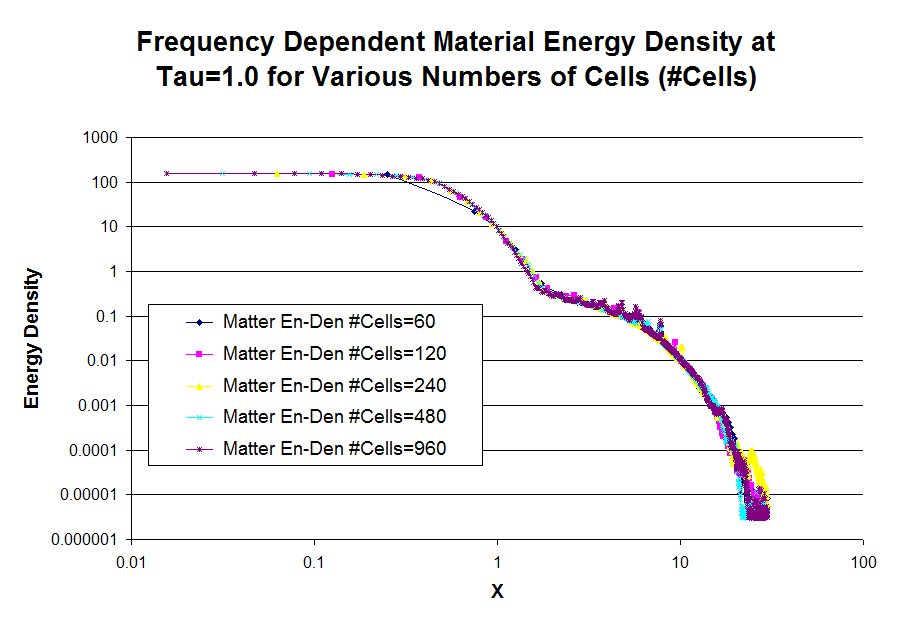
\includegraphics[width=\imgwidth,height=\imgheight]{NG-Refine-Space}}
		\end{picture}
		\caption{\label{fig:NG-Refine-Space} Frequency dependent IMD solution for various cell sizes. (Problem 3.2a)}
		\end{minipage} %\hfill
	\end{center}
\end{figure}

	Figure \ref{fig:NG-Refine-Space} shows the solution to the frequency dependent IMD method with the various spatial refinements. The solution is relatively insensitive to the choice of spatial cell size.

\begin{figure}[htbp]
	\unitlength1in
	\begin{center}
		\begin{minipage}[t]{6in}
		\centering
		\begin{picture}(\width,\height)
	                {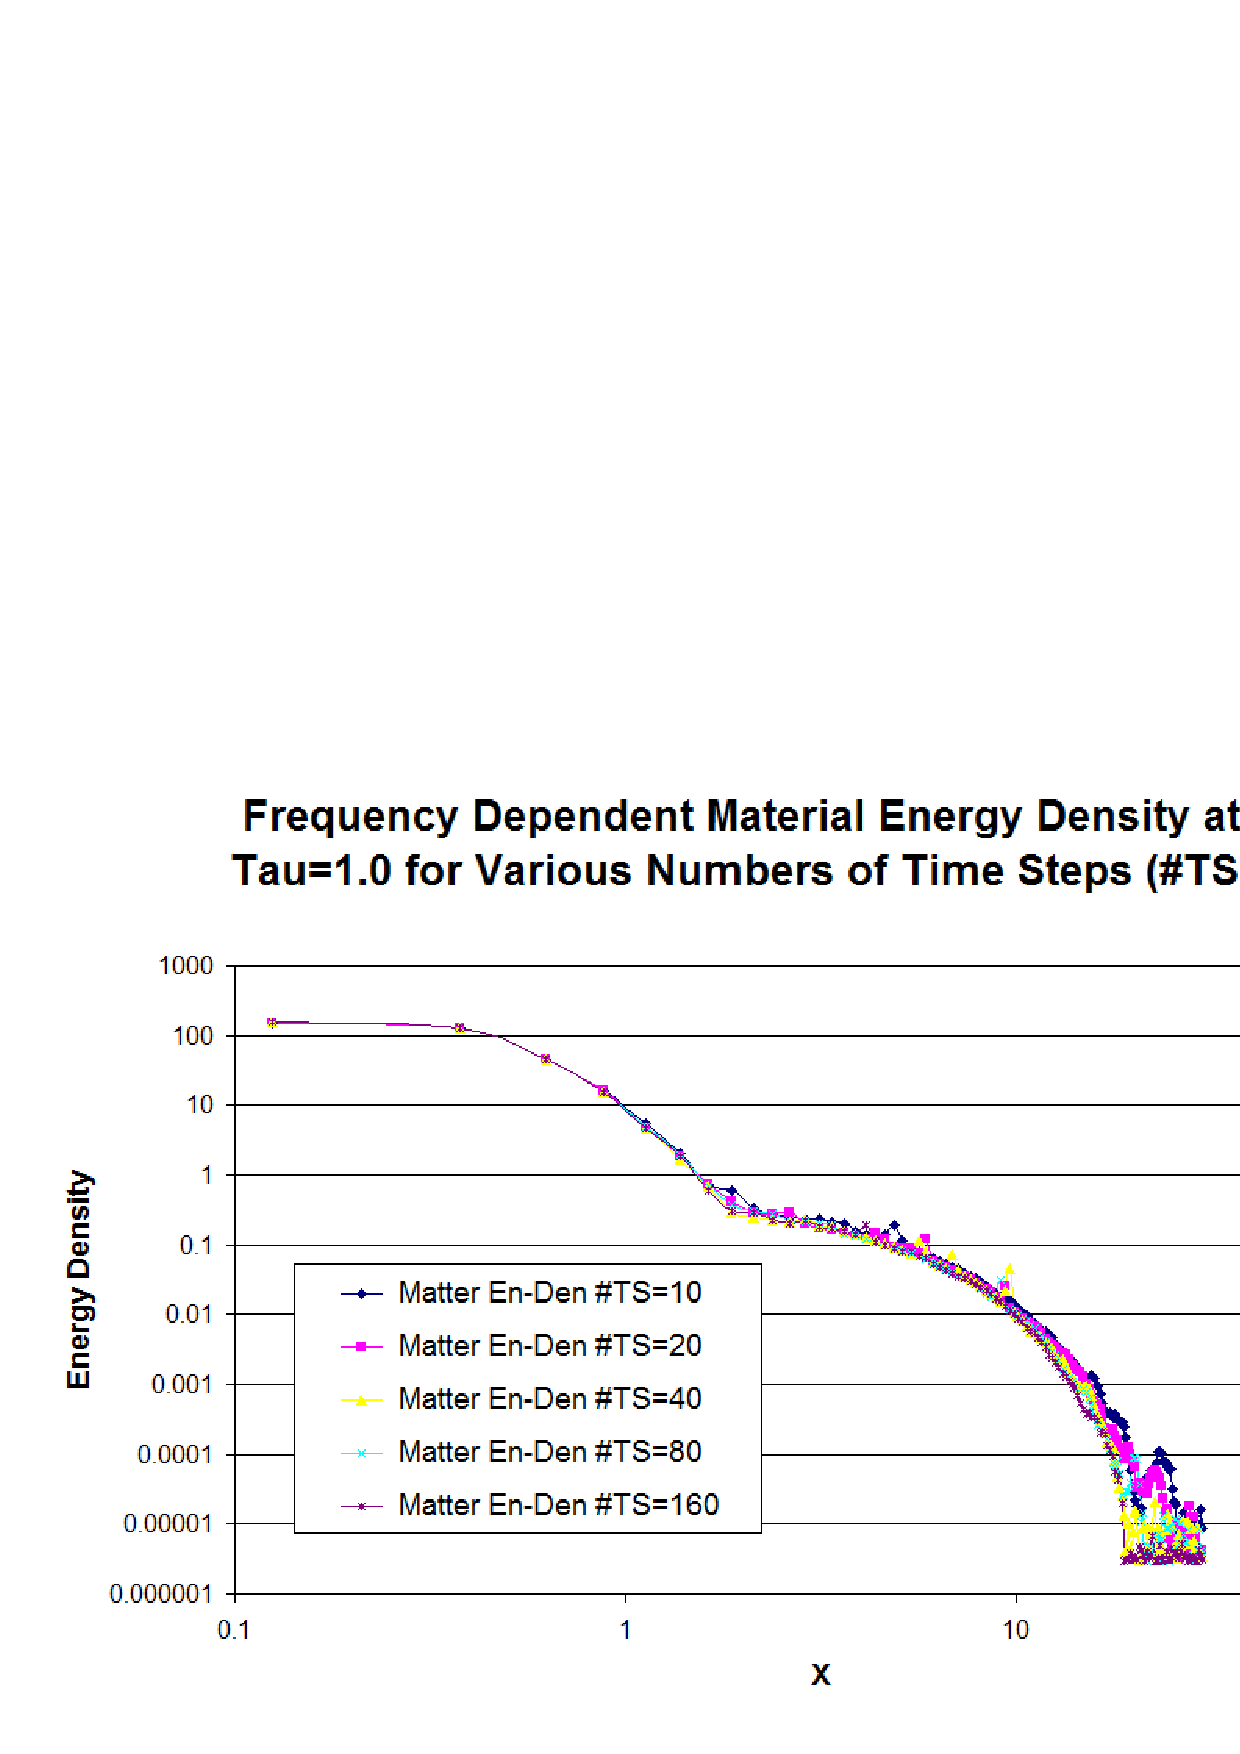
\includegraphics[width=\imgwidth,height=\imgheight]{NG-Refine-time1}}
		\end{picture}
		\caption{\label{fig:NG-Refine-time1} Frequency dependent IMD solution for various time step sizes. (Problem 3.2b)}
		\end{minipage} %\hfill
	\end{center}
\end{figure}

\begin{figure}[htbp]
	\unitlength1in
	\begin{center}
		\begin{minipage}[t]{6in}
		\centering
		\begin{picture}(\width,\height)
	                {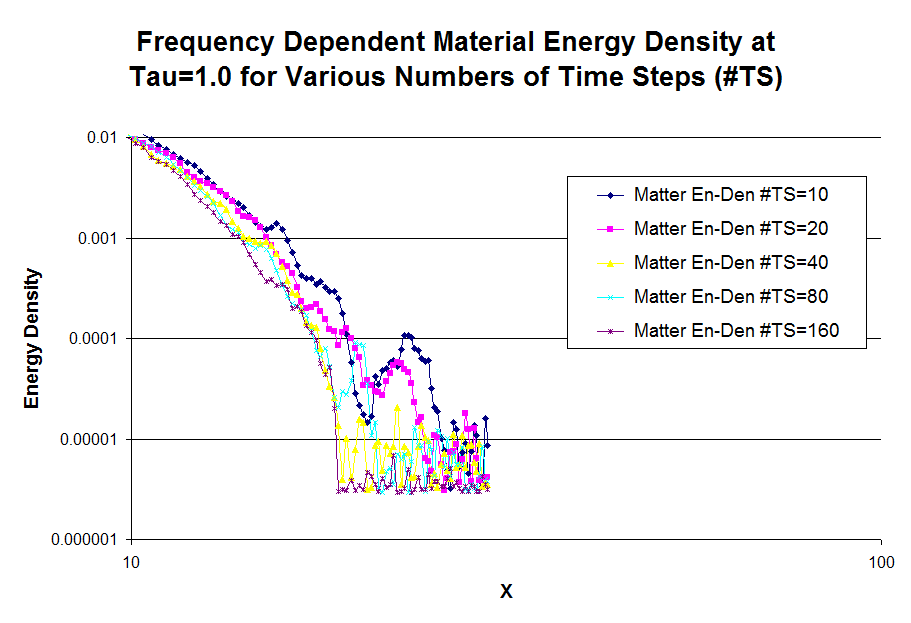
\includegraphics[width=\imgwidth,height=\imgheight]{NG-Refine-time2}}
		\end{picture}
		\caption{\label{fig:NG-Refine-time2} A closer view of the frequency dependent IMD solution for various time step sizes at the head of the Marshak wave. (Problem 3.2b)}
		\end{minipage} %\hfill
	\end{center}
\end{figure}

	Figures \ref{fig:NG-Refine-time1} and \ref{fig:NG-Refine-time2} show the dependence on the time step size. The penetration distance of the Marshak wave is influenced by the time step size. 

	The group refinement on the material energy density and the effect of frequency group calculation time was also investigated. This set of problems has the specifications in Table \ref{table:Problem3.3} with several choices of group structures: 1000 groups, 2000 groups, 4000 groups, 8000 groups, and 16000 groups. 

\begin{table}[htbp]
	\begin{center}	
	\begin{tabular} {|c||c|c|c|} \hline
		\multicolumn{3}{|c|} {Problem 3.3 Parameters} \\ [0.5ex]\hline
		Parameter & Value  & Units \\ [0.5ex] \hline\hline
		{{Number of Cells}} 	& 120 	& N/A \\ \hline
		{{Number of Particles}} & 10000 & N/A \\ \hline
		{{Length}} 		& 30 	& Mm \\ \hline
		{{Left Albedo}} 	& 1 	& N/A \\ \hline
		{{Right Albedo}} 	& 1 	& N/A \\ \hline
		{{Initial Material Temp.}} & 0.01 & K \\ \hline
		{{Material Density}} 	& 1.0 	& Kg/Mm \\ \hline
		{{Number Of Time Steps}}& 20 	& N/A \\ \hline
		{{Final Time [$\tau$]}} 	& 1.0 	& N/A \\ \hline
		{{Small Opacity}} 	& ${2\over{101}}$  & 1/Mm \\ \hline
		{{Large Opacity}} 	& ${200\over{101}}$  & 1/Mm \\ \hline
		{{Number of Groups}} 	& 1000  & 1/Mm \\ \hline	
	\end{tabular}
	\caption{\label{table:Problem3.3} Problem specifications used for the frequency dependent IMD with various numbers of groups. (Problem 3.3)}
	\end{center}
 \end{table}

\begin{figure}[htbp]
	\unitlength1in
	\begin{center}
		\begin{minipage}[t]{6in}
		\centering
		\begin{picture}(\width,\height)
	                {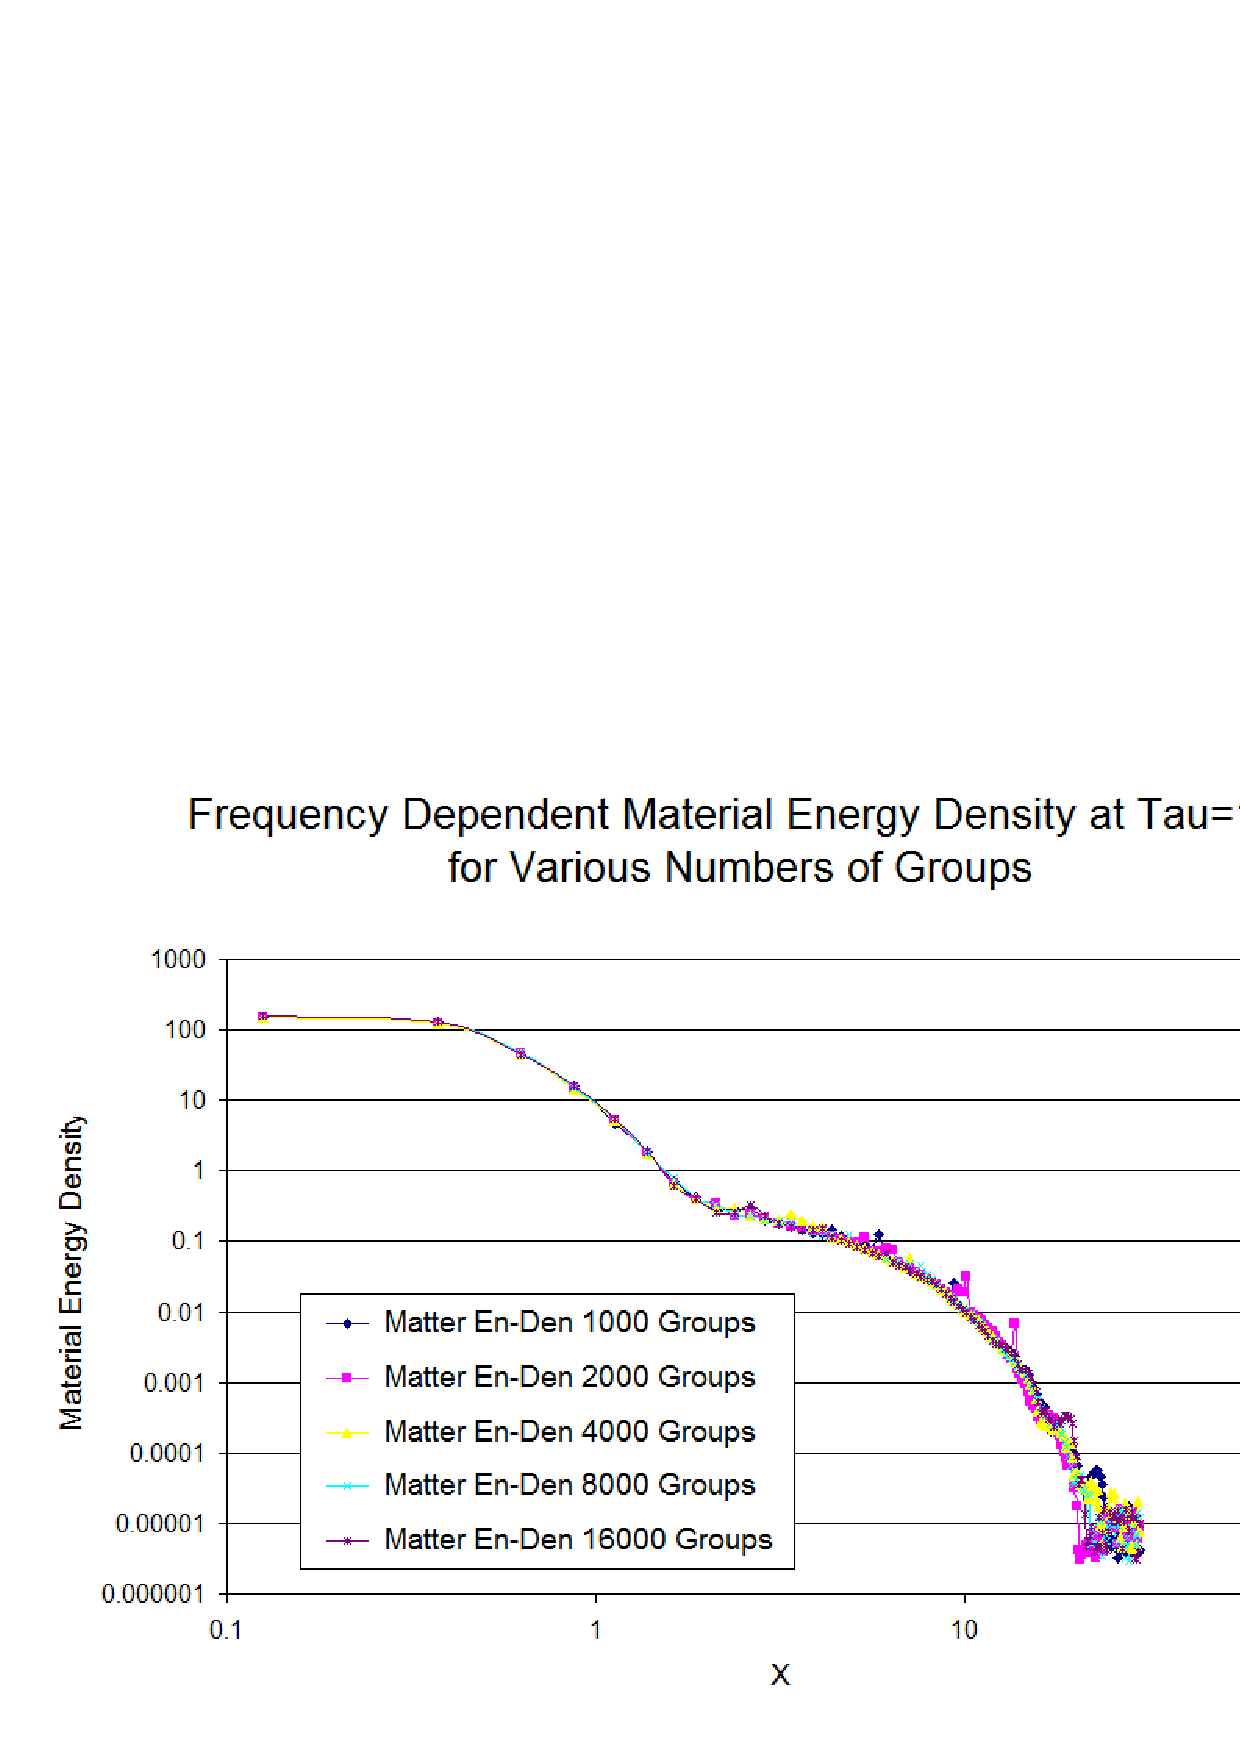
\includegraphics[width=\imgwidth,height=\imgheight]{NG-MG}}
		\end{picture}
		\caption{\label{fig:NG-MG} The material energy density determined by the frequency dependent IMD method for various numbers of groups. (Problem 3.3)}
		\end{minipage} %\hfill
	\end{center}
\end{figure}

\begin{figure}[htbp]
	\unitlength1in
	\begin{center}
		\begin{minipage}[t]{6in}
		\centering
		\begin{picture}(\width,\height)
	                {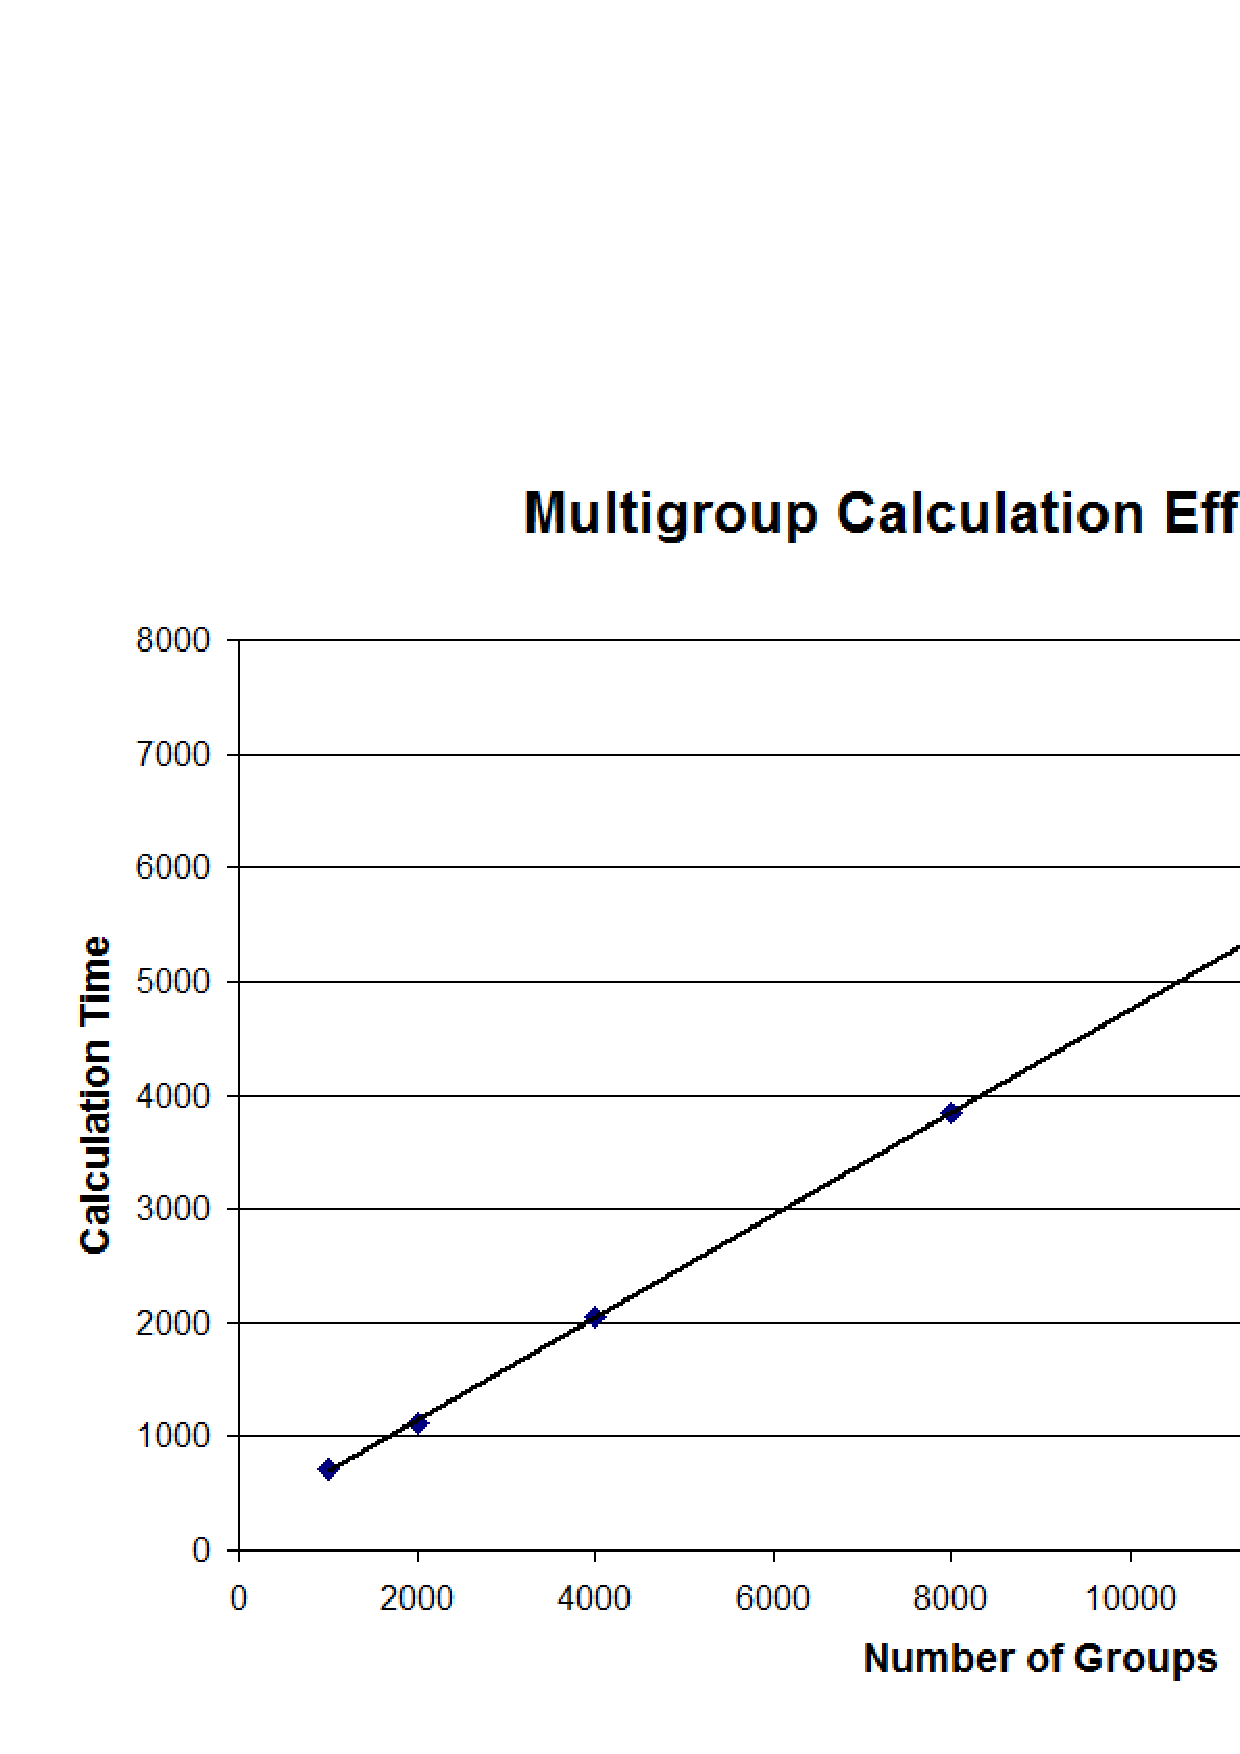
\includegraphics[width=\imgwidth,height=\imgheight]{MG_Calc_Efficiency}}
		\end{picture}
		\caption{\label{fig:MG-Calc-Efficiency} Computational cost as a function of number of groups used in the calculation (Problem 3.3)}
		\end{minipage} %\hfill
	\end{center}
\end{figure}

	The material energy density determined by the multigroup IMD method for various numbers of groups is shown in Figure \ref{fig:NG-MG}. Figure \ref{fig:MG-Calc-Efficiency} shows the computational cost as a function of numbers of groups used for the calculation.


%==================%5s
% SubSubSection:   %
%    Grey Without the Difference Formulation %
%==================%
\subsubsection{Frequency Dependent IMD with the Difference Formulation}
\label{sec:Grey_w/df}

	This section will explore properties of the frequency dependent implementation of IMD with the difference formulation. We will generate three different solutions using the IMD code with the difference formulation and one without the difference formulation. The problem specifications are listed in Table \ref{table:Problem4.1}. This problem will be referred to as ``Problem 4.1''.

\begin{table}[htbp]
	\begin{center}	
	\begin{tabular} {|c||c|c|c|} \hline
		\multicolumn{3}{|c|} {Problem 4.1 Parameters} \\ [0.5ex]\hline
		Parameter & Value  & Units \\ [0.5ex] \hline\hline
		{{Number of Cells}} 	& 500 	& N/A \\ \hline
		{{Number of Particles}} & 10000 & N/A \\ \hline
		{{Length}} 		& 50 	& Mm \\ \hline
		{{Left Albedo}} 	& 1 	& N/A \\ \hline
		{{Right Albedo}} 	& 1 	& N/A \\ \hline
		{{Initial Material Temp.}} & 0.01 & K \\ \hline
		{{Material Density}} 	& 1.0 	& Kg/Mm \\ \hline
		{{Number Of Time Steps}}& 20 	& N/A \\ \hline
		{{Final Time [$\tau$]}} & 1.0 	& N/A \\ \hline
		{{Small Opacity}} 	& ${2\over{101}}$  & 1/Mm \\ \hline
		{{Large Opacity}} 	& ${200\over{101}}$  & 1/Mm \\ \hline
	\end{tabular}
	\caption{\label{table:Problem4.1} Problem specifications used for the frequency dependent difference formulation tests. (Problem 4.1)}
	\end{center}
 \end{table}

	The temperature distribution used in the difference formulation is a user described quantity. This termperature is varied such that it was a defined percentage of the current material temperature for the associated cell. The percentages used for these problems are listed in Table \ref{table:percent-Tm}. we are interested in the effect this choice has on computational cost of the method and the degree of variance reduction.

\begin{table}[htbp]
	\begin{center}	
	\begin{tabular} {|c||c|} \hline
		\multicolumn{2}{|c|} {Difference Formulation Temperatures for Problem 4.1} \\ [0.5ex]\hline
		Problem Realization & \% Material Temperature \\ [0.5ex] \hline\hline
		 Problem 4.1a  & 00.0 \%      \\ \hline
		 Problem 4.1b  & 10.0 \%      \\ \hline
		 Problem 4.1c  & 30.0 \%      \\ \hline
		 Problem 4.1d  & 50.0 \%      \\ \hline
	\end{tabular}
	\caption{\label{table:percent-Tm} The percentages of the material temperature used for the difference formulation temperature. (Problem 4.1)}
	\end{center}
 \end{table}
	 
\begin{figure}[htbp]
	\unitlength1in
	\begin{center}
		\begin{minipage}[t]{6in}
		\centering
		\begin{picture}(\width,\height)
	                {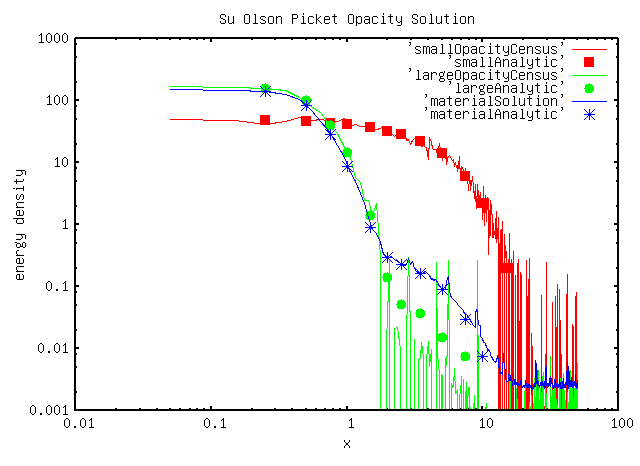
\includegraphics[width=\imgwidth,height=\imgheight]{NG-NDF}}
		\end{picture}
		\caption{\label{fig:NG-NDF} Frequency dependent result without the difference formulation compared to the Su and Olson semi-analytic result[Su 1999]. (Problem 4.1a) }
		\end{minipage} %\hfill
	\end{center}
\end{figure}

\begin{figure}[htbp]
	\unitlength1in
	\begin{center}
		\begin{minipage}[t]{6in}
		\centering
		\begin{picture}(\width,\height)
	                {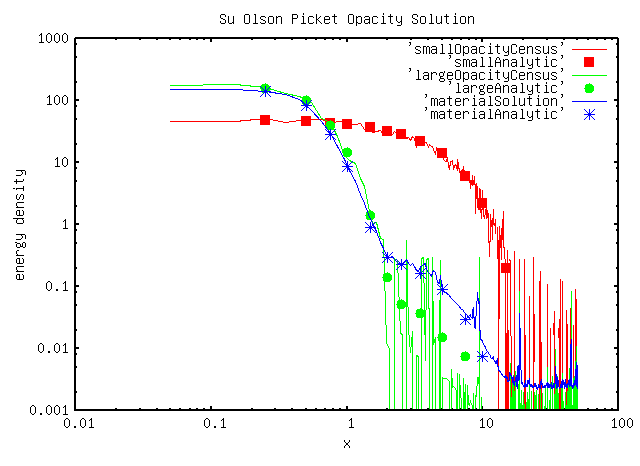
\includegraphics[width=\imgwidth,height=\imgheight]{NG-DF-10}}
		\end{picture}
		\caption{\label{fig:NG-DF-10} Frequency dependent result, using the difference formulation temperature set to 10\% of the material temperature, compared to the Su and Olson semi-analytic result[Su 1999]. (Problem 4.1b) }
		\end{minipage} %\hfill
	\end{center}
\end{figure}

\begin{figure}[htbp]
	\unitlength1in
	\begin{center}
		\begin{minipage}[t]{6in}
		\centering
		\begin{picture}(\width,\height)
	                {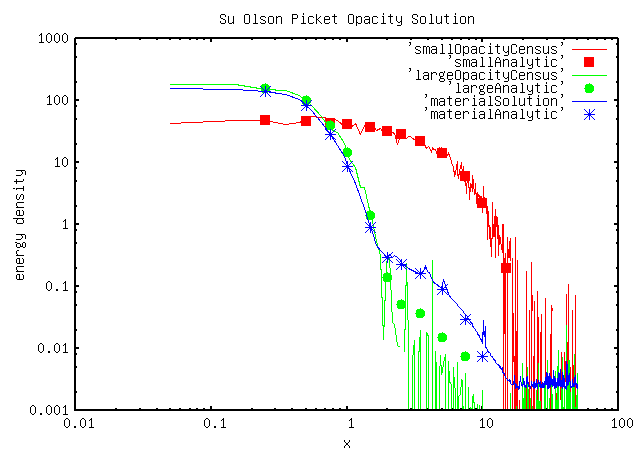
\includegraphics[width=\imgwidth,height=\imgheight]{NG-DF-30}}
		\end{picture}
		\caption{\label{fig:NG-DF-30} Frequency dependent result, using the difference formulation temperature set to 30\% of the material temperature, compared to the Su and Olson semi-analytic result[Su 1999]. (Problem 4.1c) }
		\end{minipage} %\hfill
	\end{center}
\end{figure}

\begin{figure}[htbp]
	\unitlength1in
	\begin{center}
		\begin{minipage}[t]{6in}
		\centering
		\begin{picture}(\width,\height)
	                {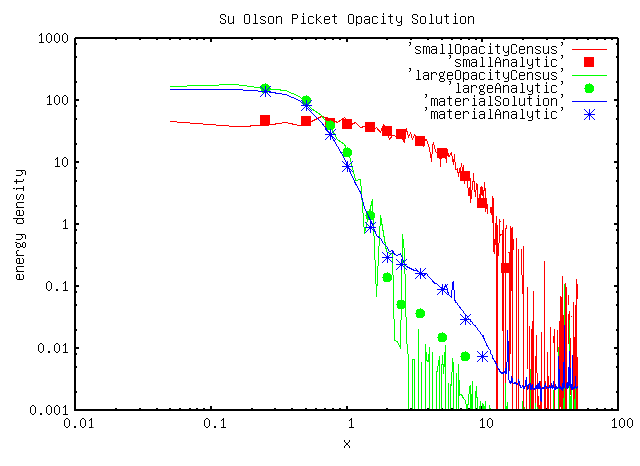
\includegraphics[width=\imgwidth,height=\imgheight]{NG-DF-50}}
		\end{picture}
		\caption{\label{fig:NG-DF-50} Frequency dependent result, using the difference formulation temperature set to 50\% of the material temperature, compared to the Su and Olson semi-analytic result[Su 1999]. (Problem 4.1d) }
		\end{minipage} %\hfill
	\end{center}
\end{figure}

	Figures \ref{fig:NG-NDF}, \ref{fig:NG-DF-10}, \ref{fig:NG-DF-30}, and \ref{fig:NG-DF-50} show the IMD solution with the difference formulation for the various percentages of the difference formulation temperature as compared to the material temperature. The ``smallAnalytic'', ``largeAnalytic'', and ``materialAnalytic'' denote the Su and Olson semi-analytic non-grey benchmark results for the energy density of the small opacity associated photons, large opacity associated photons, and the material, respectively. The material energy density results are displayed for all four realizations of Problem 4.1 in figure \ref{fig:DF-NG-MaterialEnergyDensity}.

\begin{figure}[htbp]
	\unitlength1in
	\begin{center}
		\begin{minipage}[t]{6in}
		\centering
		\begin{picture}(\width,\height)
	                {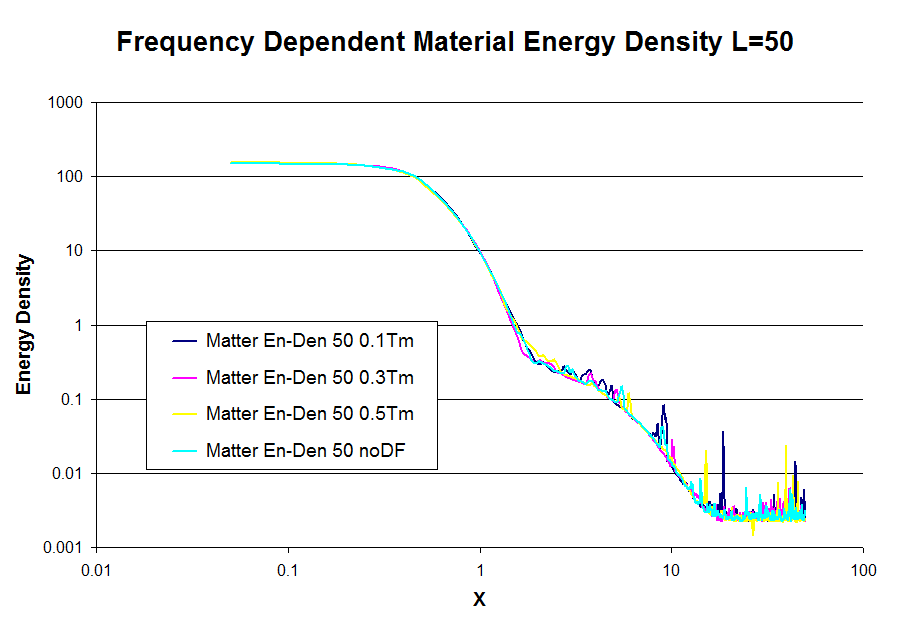
\includegraphics[width=\imgwidth,height=\imgheight]{DF-NG-MaterialEnergyDensity}}
		\end{picture}
		\caption{\label{fig:DF-NG-MaterialEnergyDensity} Non-grey result at various percentages of the material temperature for the difference formulation. (Problem 4.1)}
		\end{minipage} %\hfill
	\end{center}
\end{figure}


	The relative standard deviations associated with the material energy density for the different realizations of Problem 4.1 are shown in Figure \ref{fig:DF-NG-RelSTD50}. The relative standard deviation is simply the standard deviation of the associated cell energy density divided by the value of the energy density in that cell. 

\begin{figure}[htbp]
	\unitlength1in
	\begin{center}
		\begin{minipage}[t]{6in}
		\centering
		\begin{picture}(\width,\height)
	                {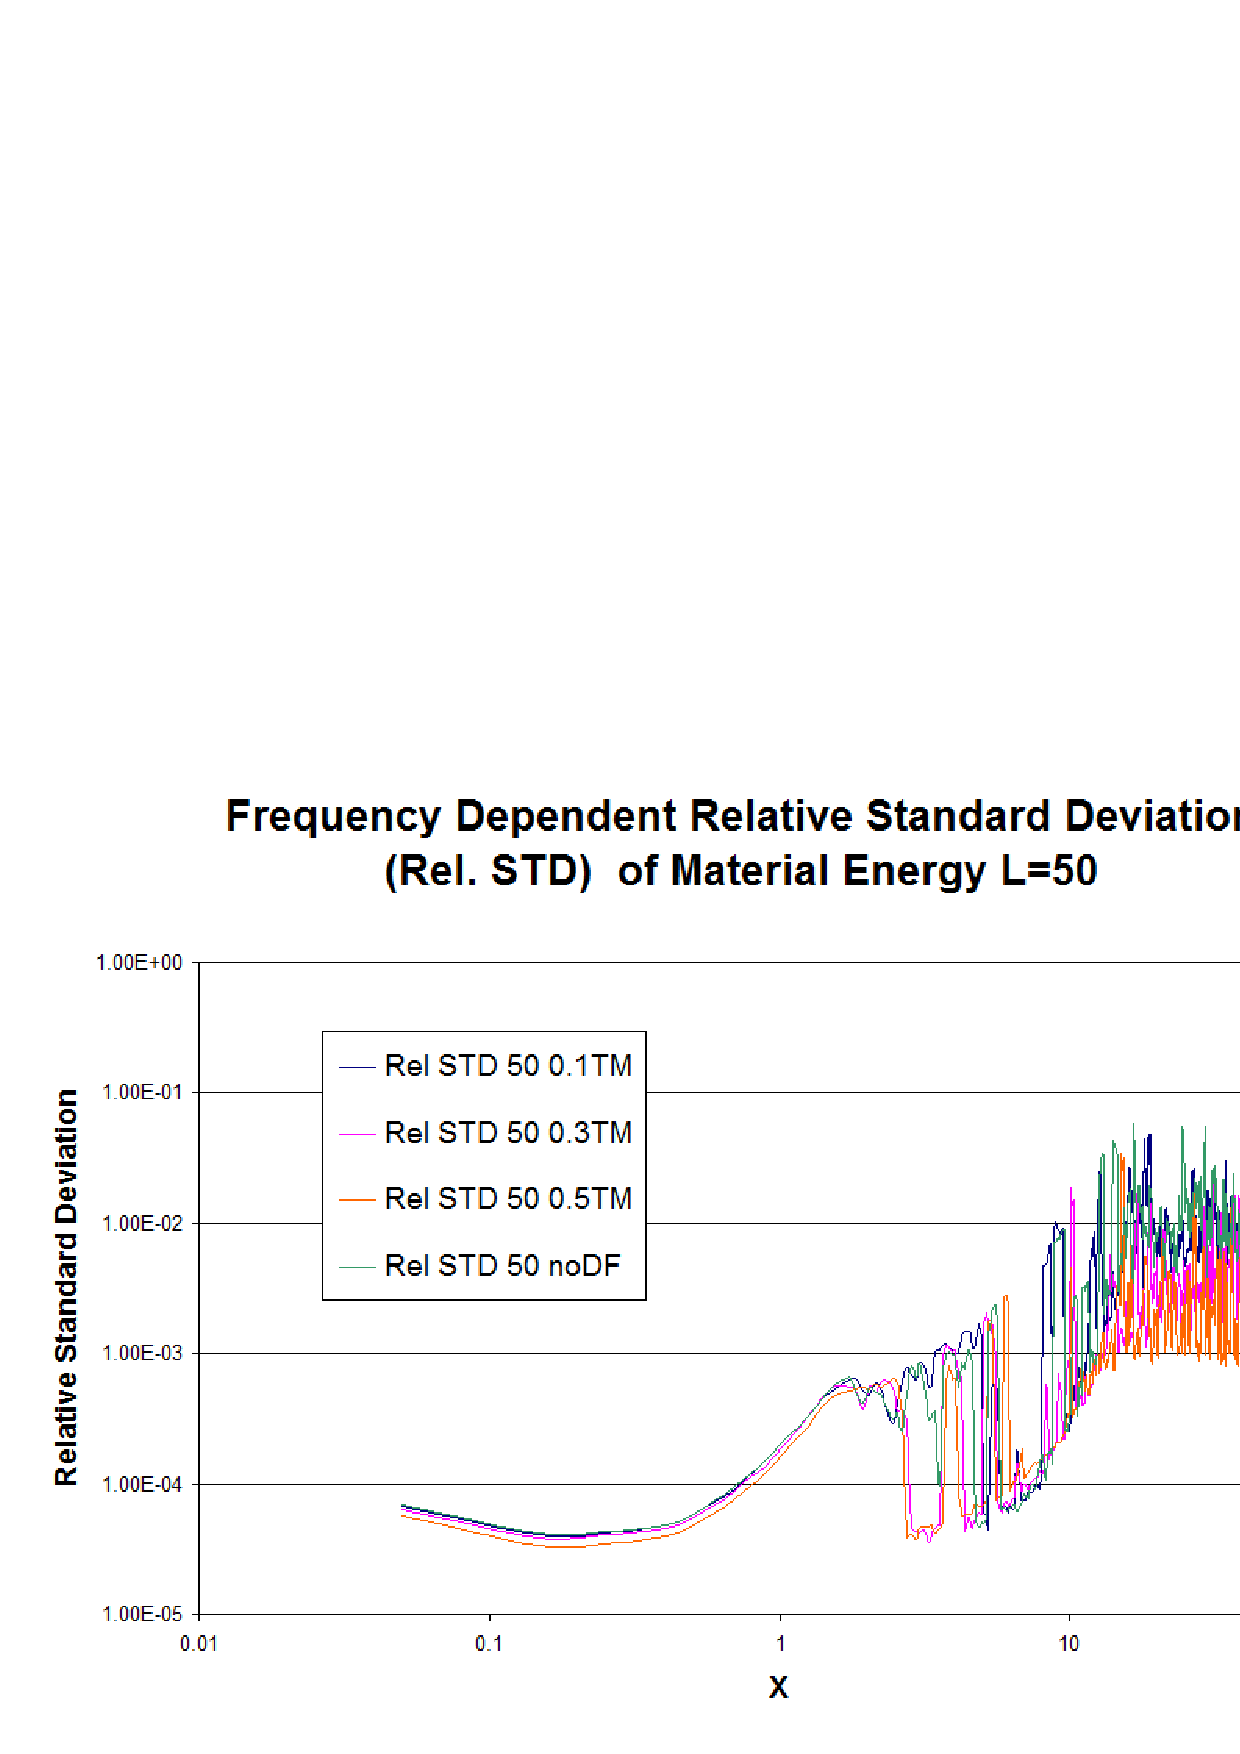
\includegraphics[width=\imgwidth,height=\imgheight]{DF-NG-RelSTD50}}
		\end{picture}
		\caption{\label{fig:DF-NG-RelSTD50} The relative standard deviation of the material energy density for the different realization of Problem 4.1.}
		\end{minipage} %\hfill
	\end{center}
\end{figure}

	In Figure \ref{fig:DF-NG-RelSTD50}, the values associated with ``Rel STD 50 0.1Tm'' denotes the relative standard deviation (Rel STD) of the material energy density with total problem length equal to 50 Mm and the difference formulation temperature equal to 10\% of the material temperature. The other values are defined similarly with the exception of ``Rel STD 50 noDF'' which denotes the solution generated without the difference formulation. 

% 	The figure of merit of each cell's material energy density can be calculated as ${1\over{\sigma^2t}}$ where $\sigma^2$ denotes the variance of the material energy density and $t$ denotes the calculation time. The relative figure of merit is defined for this work as the figure of merit of the material energy density with the difference formulation divided by the figure of merit without the difference formulation for an associated cell. This value can be used to determine the effective decrease in variance as a function of the computational cost. 
% 
% \begin{figure}[htbp]
% 	\unitlength1in
% 	\begin{center}
% 		\begin{minipage}[t]{6in}
% 		\centering
% 		\begin{picture}(\width,\height)
% 	                {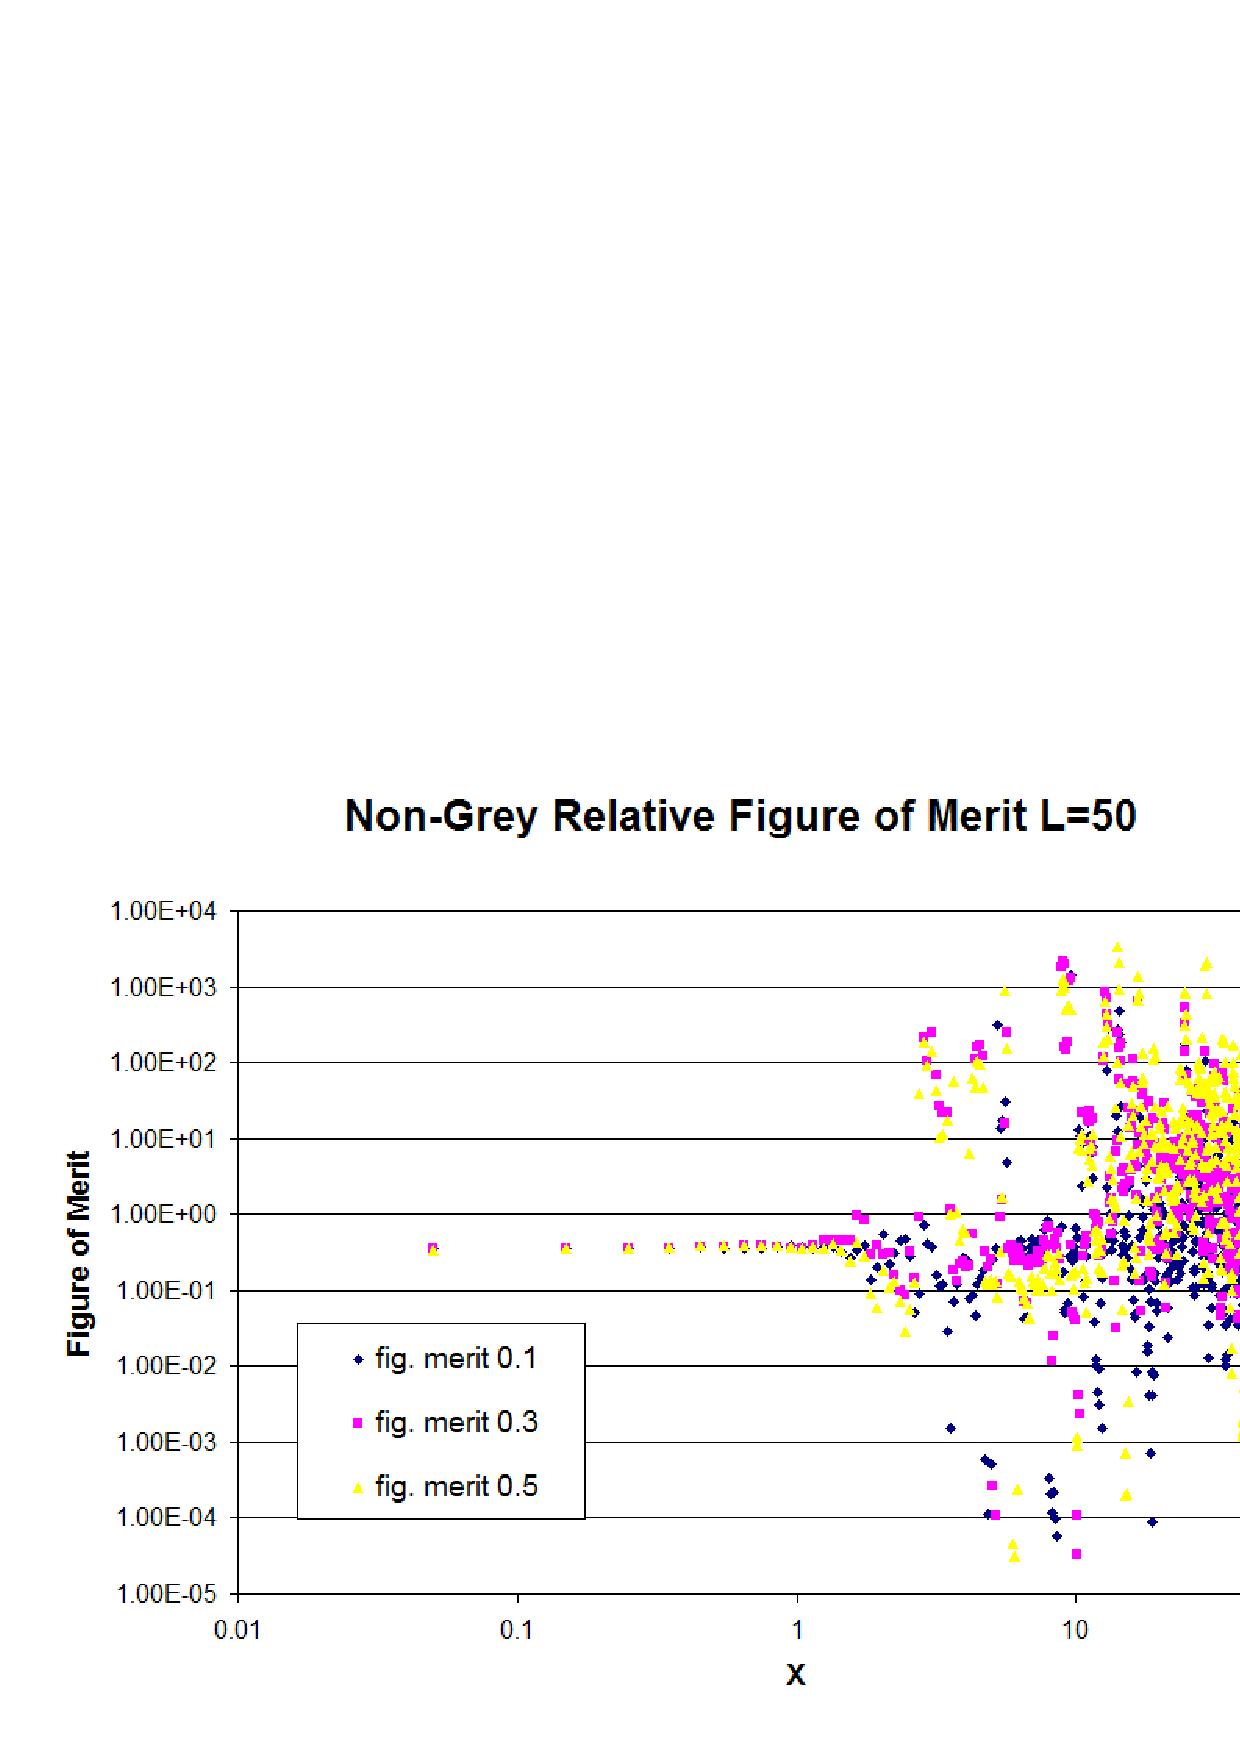
\includegraphics[width=\imgwidth,height=\imgheight]{DF-NG-FigMerit50}}
% 		\end{picture}
% 		\caption{\label{fig:DF-NG-FigMerit50} The relative figure of merit per cell for the difference formulation at various percentages of the material temperature. (Problem 4.1)}
% 		\end{minipage} %\hfill
% 	\end{center}
% \end{figure}
% 		
% 	In Figure \ref{fig:DF-NG-FigMerit50}, it is important to note that this expresses the figure of merit at each cell which is determined from the variance in the associated cell and the total computation time of the problem. It is also important to note that any value of relative figure of merit below one or greater than one demonstrate a relative decrease or increase in the comparative figure of merit respectively.

	For Problem 4.1 the total figure of merit is the sum of the figure of merit for each cell over the whole problem. The associated relative total figure of merit is the total figure of merit associated with a given variance reduction technique divided by the total figure of merit without it. This is expressed for Problem 4.1 in Figure \ref{fig:DF-NG-TotalFigMerit}.

\begin{figure}[htbp]
	\unitlength1in
	\begin{center}
		\begin{minipage}[t]{6in}
		\centering
		\begin{picture}(\width,\height)
	                {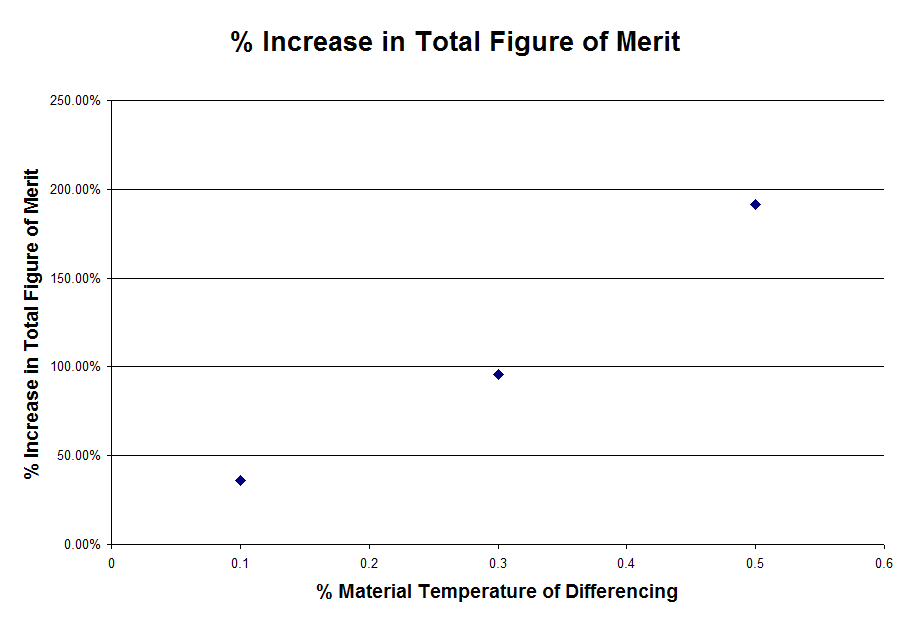
\includegraphics[width=\imgwidth,height=\imgheight]{DF-NG-TotalFigMerit}}
		\end{picture}
		\caption{\label{fig:DF-NG-TotalFigMerit} The relative total figure of merit for the difference formulation at various percentages of the material temperature. (Problem 4.1)}
		\end{minipage} %\hfill
	\end{center}
\end{figure}

% 	Similarly, for Problem 4.1 the average figure of merit is the average figure of merit in each cell over the whole problem. The associated relative average figure of merit is the relative average figure of merit associated with a given variance reduction technique divided by the relative average figure of merit without it. This is expressed for Problem 4.1 in Figure \ref{fig:DF-NG-AveFigMerit}.
% 
% \begin{figure}[htbp]
% 	\unitlength1in
% 	\begin{center}
% 		\begin{minipage}[t]{6in}
% 		\centering
% 		\begin{picture}(\width,\height)
% 	                {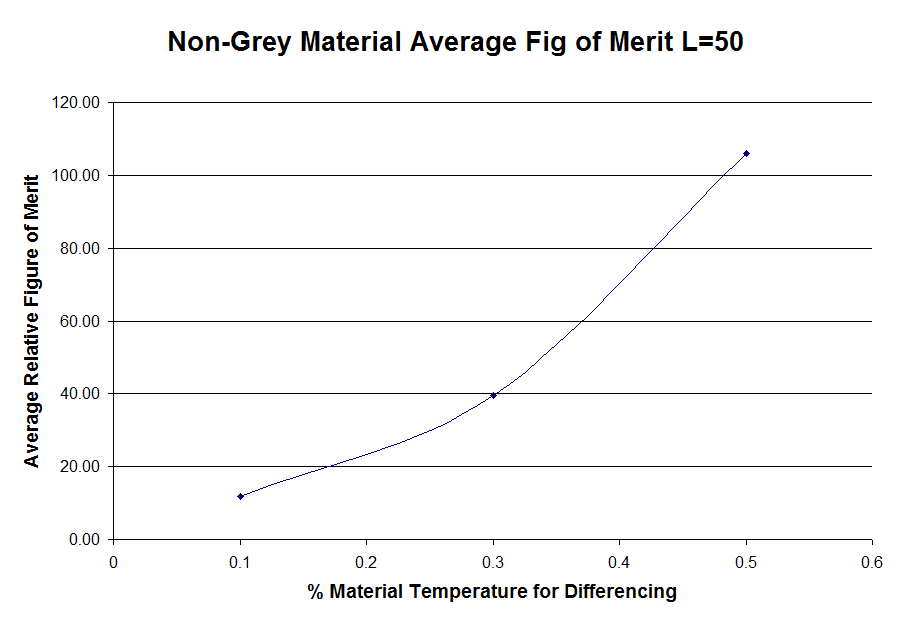
\includegraphics[width=\imgwidth,height=\imgheight]{DF-NG-AveFigMerit}}
% 		\end{picture}
% 		\caption{\label{fig:DF-NG-AveFigMerit} The relative average figure of merit for the difference formulation at various percentages of the material temperature. (Problem 4.1)}
% 		\end{minipage} %\hfill
% 	\end{center}
% \end{figure}

\belowSubSecSkip

%=====================================================================%
% SubSection:                        	                              %
%     Results: Summary %
%=====================================================================%
\subsection{Summary}
\label{sec:Results-Summary}

\noindent
	\indent The results obtained from the grey and frequency dependent calculations were compared to the benchmark semi-analytic results of Su and Olson[Su 1996][Su 1999], with and without the difference formulation. The temporal and spatial resolution dependence was tested for both the grey and frequency dependent IMD methods using five refinements in each independent variable.  The efficiency of the difference formulation at various percentages of the material temperature was tested as a way to reduce the material energy density variance.











